\documentclass[usenatbib]{mn2e}
\usepackage{amsmath} 
\usepackage{amssymb} 
\usepackage{graphics}
\usepackage{graphicx}
\usepackage{epsfig}  
\def\be{\begin{equation}}
\def\ee{\end{equation}}
\def\ba{\begin{eqnarray}}
\def\ea{\end{eqnarray}}

\newcommand{\documentname}{paper~}
\newcommand{\match}{{\tt match}~}
\newcommand{\apj}{ApJ}  
\newcommand{\apjs}{ApJS}  
\newcommand{\apjl}{ApJL}  
\newcommand{\aj}{AJ}  
\newcommand{\mnras}{MNRAS}  
\newcommand{\mnrassub}{MNRAS accepted}  
\newcommand{\aap}{A\&A}  
\newcommand{\aaps}{A\&AS}  
\newcommand{\araa}{ARA\&A}  
\newcommand{\nat}{Nature}  
\newcommand{\physrep}{PhR}
\newcommand{\pasp}{PASP}    
\newcommand{\pasj}{PASJ}    

\newcommand{\kms}{\,km~s$^{-1}$}
\def\squig{\sim\!\!}
\newcommand{\LCDM}{$\Lambda$CDM~}
\newcommand{\beq}{\begin{eqnarray}}  
\newcommand{\eeq}{\end{eqnarray}}   
\newcommand{\zz}{$z\sim 3$} 
\newcommand{\avg}[1]{\langle{#1}\rangle}  
\newcommand{\ly}{{\ifmmode{{\rm Ly}\alpha}\else{Ly$\alpha$~}\fi}}
\newcommand{\hMpc}{{\ifmmode{h^{-1}{\rm Mpc}}\else{$h^{-1}$Mpc }\fi}}  
\newcommand{\hGpc}{{\ifmmode{h^{-1}{\rm Gpc}}\else{$h^{-1}$Gpc }\fi}}  
\newcommand{\hmpc}{{\ifmmode{h^{-1}{\rm Mpc}}\else{$h^{-1}$Mpc }\fi}}  
\newcommand{\hkpc}{{\ifmmode{h^{-1}{\rm kpc}}\else{$h^{-1}$kpc }\fi}}  
\newcommand{\hMsun}{{\ifmmode{h^{-1}{\rm
        {M_{\odot}}}}\else{$h^{-1}{\rm{M_{\odot}}}$}\fi}}   
\newcommand{\hmsun}{{\ifmmode{h^{-1}{\rm
        {M_{\odot}}}}\else{$h^{-1}{\rm{M_{\odot}}}$}\fi}}   
\newcommand{\Msun}{{\ifmmode{{\rm {M_{\odot}}}}\else{${\rm{M_{\odot}}}$}\fi}}  
\newcommand{\msun}{{\ifmmode{{\rm {M_{\odot}}}}\else{${\rm{M_{\odot}}}$}\fi}}  
\newcommand{\clara}{{\texttt{CLARA}}~}
\newcommand{\rand}{{\ifmmode{{\mathcal{R}}}\else{${\mathcal{R}}$ }\fi}}  
\newcommand{\Lsun}{\mbox{\,$L_{\odot}$}}
\newcommand{\like}{\mathscr{L}}
\newcommand{\bftheta}{\mathbf{\Theta}}
\newcommand{\degree}{\ensuremath{^\circ}}
\def\spose#1{\hbox to 0pt{#1\hss}}
\def\simlt{\mathrel{\spose{\lower 3pt\hbox{$\mathchar"218$}}
     \raise 2.0pt\hbox{$\mathchar"13C$}}}
\def\simgt{\mathrel{\spose{\lower 3pt\hbox{$\mathchar"218$}}
     \raise 2.0pt\hbox{$\mathchar"13E$}}}
\font\smcap=cmcsc10

\begin{document}

\title[Halo mass and occupation fraction of LAEs at$z=3.1$]{Mass and
  occupation fraction of dark matter halos hosting Lyman-$\alpha$
  emitters at $z\sim 3$}      
\author[~J.~E. Forero-Romero and ~J.~E. Mejia-Restrepo]{
\parbox[t]{\textwidth}{\raggedright 
  Jaime E. Forero-Romero$^{1}$ and
  Julian E. Mej\'ia-Restrepo$^{2}$ 
}
\vspace*{6pt}\\
$^{1}$ Departamento de F\'{i}sica, Universidad de los Andes, Cra. 1
No. 18A-10, Edificio Ip, Bogot\'a, Colombia \\
$^{2}$ Departamento de Astronom\'{i}a, Universidad de Chile, Camino el
Observatorio 1515, Santiago, Chile} 

\maketitle

\begin{abstract}
%
We derive constraints on the mass and occupation fraction of dark
matter halos hosting \ly Emitting galaxies (LAEs) at a redshift of
$z=3.1$ by matching the number density distribution and the angular
correlation function between mock and observed fields. We explicitly
take into account the cosmic variance on the typical observed field
size by constructing mock fields from a large cosmological N-body
simulation with the same geometry of observed fields. To populate the
halos in the simulation we use a model where a dark matter halo with
mass in the range $M_{\rm min}<M_{\rm h}<M_{\rm max}$ can only host
one detectable LAE with a probability $0.1 \leq f_{\rm occ}\leq
1.0$. We avoid the large uncertainties in the estimation of \ly
luminosities with this approach. Our main result is that the
clustering and number density information are insufficient to impose a
tight constraint on the {\bf   occupation} fraction. On the other hand
the minimum mass and maximum mass can be constrained to the range $M_{\rm max}<10^{12}$\hMsun and $10^{10}\hMsun\leq M_{\rm min}\leq
10^{11.5}\hMsun$.  We also find that the consistent models have a narrow mass
range, $\Delta M \equiv \log_{10}M_{\rm max} - \log_{10} M_{\rm min}$,
smaller than $1.0$ dex, with a vast majority in the range $\Delta
M<0.5$ dex. {\bf These mass ranges are a sub-set of already published
constraints, while the wide range of values for the escape fraction
  are a novel result}. There is an inconclusive response as to
which is the occupation fraction for LAEs at $z=3.1$. A precise answer
requires observations on larger fields and robust physical models for
the connection between dark matter, star formation and the escape of
\ly radiation. That kind of modeling should also be able to provide a
plausible explanation for the narrow range in mass $\Delta M<1.0$ dex
derived here for the halos hosting LAEs at $z=3.1$.     

\end{abstract}

\begin{keywords}
{cosmology: theory – cosmology: large-scale structure of universe –
  galaxies: formation – galaxies: high-redshift – galaxies: statistics
  – galaxy: haloes} 
\end{keywords}


\section{Introduction}

Lyman-$\alpha$ emitting galaxies (LAEs) are helpful in a diverse range
of subjects in extragalactic astronomy. LAEs can be
used as probes of reionization \citep{Dijkstra11}, tracers of large
scale structure \citep{Koehler2007},  signposts for low metallicity
stellar populations, markers of the galaxy formation process at high
redshift \citep{Dayal2009,ForeroRomero2012} and tracers of active star
formation \citep{Guaita2013}. 

Capitalizing LAEs observations requires an understanding of
their place in the context of a given structure formation model in a
cosmological context. Under the current paradigm the dominant matter
content of the Universe is to be found in dark matter (DM) and each
galaxy is thought to be hosted by larger dark matter structure known
as a halo. \citep{Peebles1980,SpringelNature05}. 

Galaxy formation models find that halo mass predicts with high
accuracy galactic properties such as stellar mass and star formation
rate \citep{Behroozi2013a}. This suggests that the
physical processes that regulate the star formation cycle are 
dependent on halo mass.  For that reason, finding the typical dark
matter halo mass hosting LAEs represents an advance to understand the
nature of this galaxy population in the context of Lambda Cold Dark
Matter ($\Lambda$CDM) paradigm.  

Some theoretical attempts to solve this problem using an  ab-initio
approach. They start from the DM halo population to infer the
intrinsic star formation rates and \ly a luminosities. From these
values they estimate the amount of \ly photons that
escape each galaxy and compute the observed luminosity for each
galaxy. These models can predict different observables including: the
luminosity function, correlation function and the equivalent width
distributions. Such modelling has been implemented in semi-analytic
models \citep{Garel2012,Orsi2012,Soler2012} and  full N-body
hydrodynamical simulations \citep{Laursen2007, Dayal2009,
  ForeroRomero2011, Yajima2012}. 

These calculations involve many uncertain steps, such as the treatment
of astrophysical processes describing star formation. However, in the
context of LAEs, the dominant uncertainty is the estimation of the
escape fraction, that is the fraction of \ly photons that escape the
galaxy to the observer. Given the resonant nature of the \ly line, the escape
fraction is sensitive to  the dust contents, density, temperature, topology and
kinematics of the neutral Hydrogen in the interstellar medium
(ISM). Solving the radiative transfer of \ly photons in the ISM requires Monte
Carlo simulations. The process of finding a consensus on the expected
value for the \ly escape fraction in high redshift galaxies is still
matter of ongoing research
\citep{Neufeld1991,Verhamme2006,ForeroRomero2011,Dijkstra2012,Laursen2013,Orsi2012}.  

A different approach to infer the typical mass of halos hosting
LAEs is based on the spatial clustering information. This approach uses the fact
that in CDM cosmologies the spatial clustering of galaxies on large
scales is entirely dictated by the halo distribution
\citep{Colberg00}, which in turn has a strong dependence on halo
mass. Using measurements of the angular correlation function of LAEs,
observers have put constraints on the typical mass and occupation
fraction of the putative halos hosting these galaxies
\citep{Hayashino2004,Gawiser07,Nilsson2007,Ouchi2010}. In these
studies the observations are done on fields of $\sim 1$ deg$^{2}$ and
the conclusions derived on the halo host mass do not delve too deeply
into the possible impact of cosmic variance.  

Recently \cite{Yamada2012} observed a wide area of $2.4$ deg$^{2}$
under homogeneous instrumental and data reduction conditions. This data
set is constructed from 12 different sub-fields that allows us to use
clustering statistics and cosmic variance to constraint the mass and
occupation fraction of halos hosting LAEs. 

Our method first populates DM halos in cosmological simulations with
LAEs. We only consider whether a DM can host a detectable LAE or not
without predicting a \ly  luminosity. This bypasses all the physical
uncertainties involved in the estimation of observed \ly luminosities.
Once we have the mock LAE catalogs, we compare them against
observations in terms of the  statistics on the number density
distribution derived from the observations over the 12 fields of
\cite{Yamada2012}. We also use measurements of the angular
correlation function to improve these constraints. This method allows
us to constraint the preferred mass range and occupation fraction of DM
halos hosting LAEs.  
 

This \documentname is structured as follows. In the next section we present
the simulation and the model used to produce the mock catalogs. We
also list the criteria used to compare the mocks against
observations. In \S \ref{sec:results} we present the main results for
the halo mass and occupation fraction. We continue with a discussion
of these results under the light of other observational and
theoretical results. Finally, we present our conclusions in \S
\ref{sec:conclusions}.  

Throughout this \documentname we assume a $\Lambda$CDM cosmology with the
following values for the cosmological parameters, $\Omega_{m}=0.27$,
$\Omega_{\Lambda}=0.73$ and $h=0.70$, corresponding to the matter
density, vacuum density and the Hubble constant in units of 100 km
s$^{-1}$ Mpc$^{-1}$. 

\section{Methodology}


Our method is based on the comparison of observations and mock
catalogs. We use two different kinds of statistics to perform the
comparison: (i) the distribution of the surface number density
across fields and (ii) the angular correlation function.

In the next subsections we describe in detail the four key
elements int our work-flow. First we present (in two sub-sections) the
observations we take as a benchmark. Second, we describe the main
characteristics of the N-body simulation and the halo catalogs we
use. Third, we recount the important parameters of the simplified
model that we use to populate the halo catalogs with LAEs. Finally, we
describe some of the statistical tests we adopt to compare
observations and mocks .

\subsection{Observational constraints}


\begin{figure*}
\begin{center}
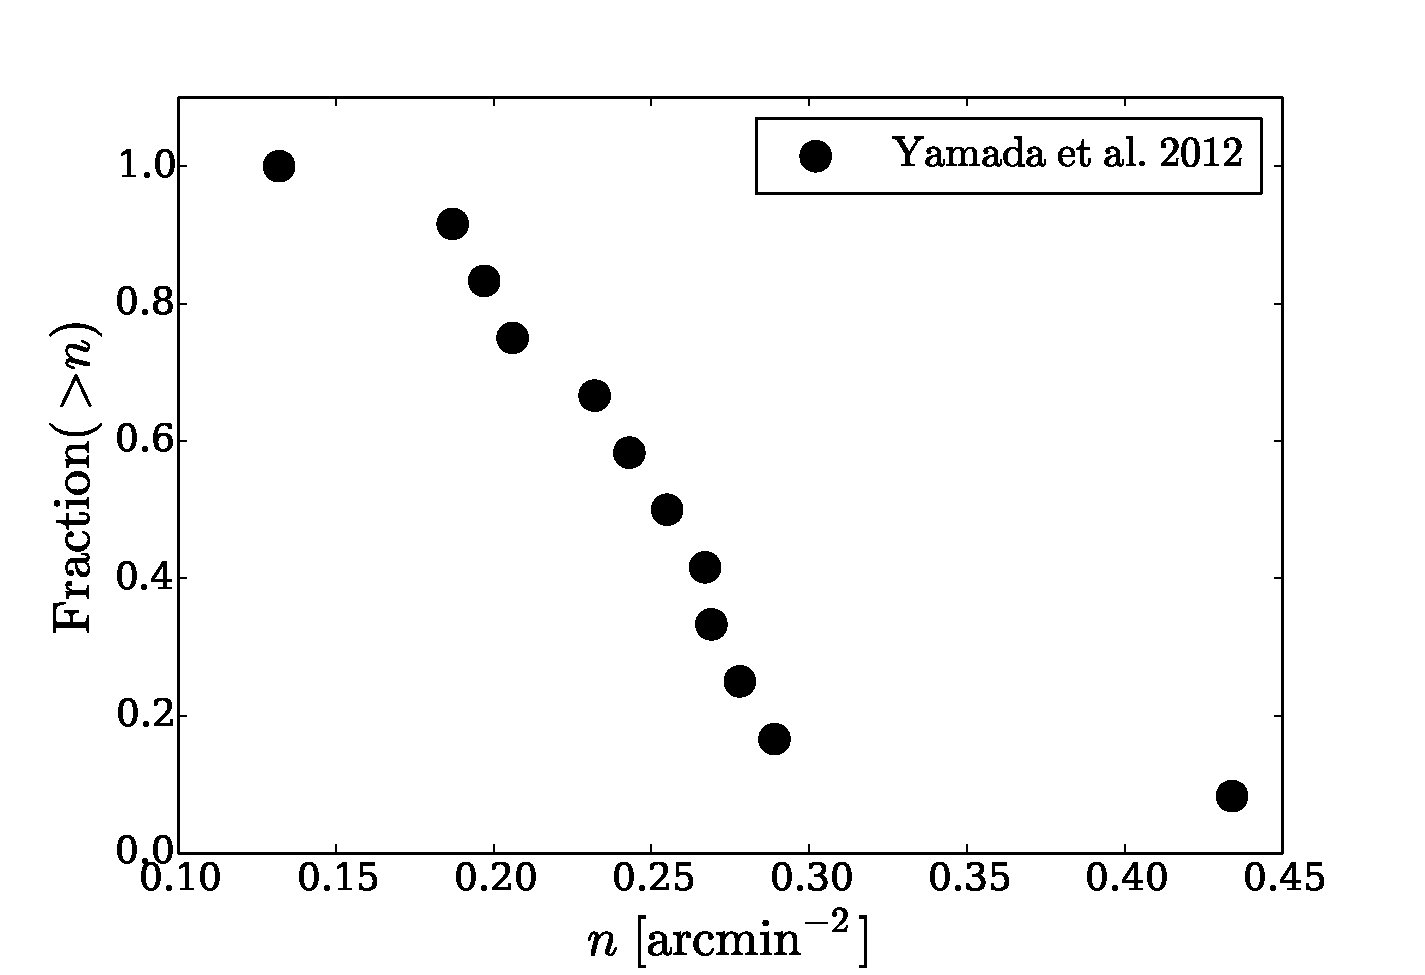
\includegraphics[width=0.45\linewidth,angle=0]{Fig1b.pdf}
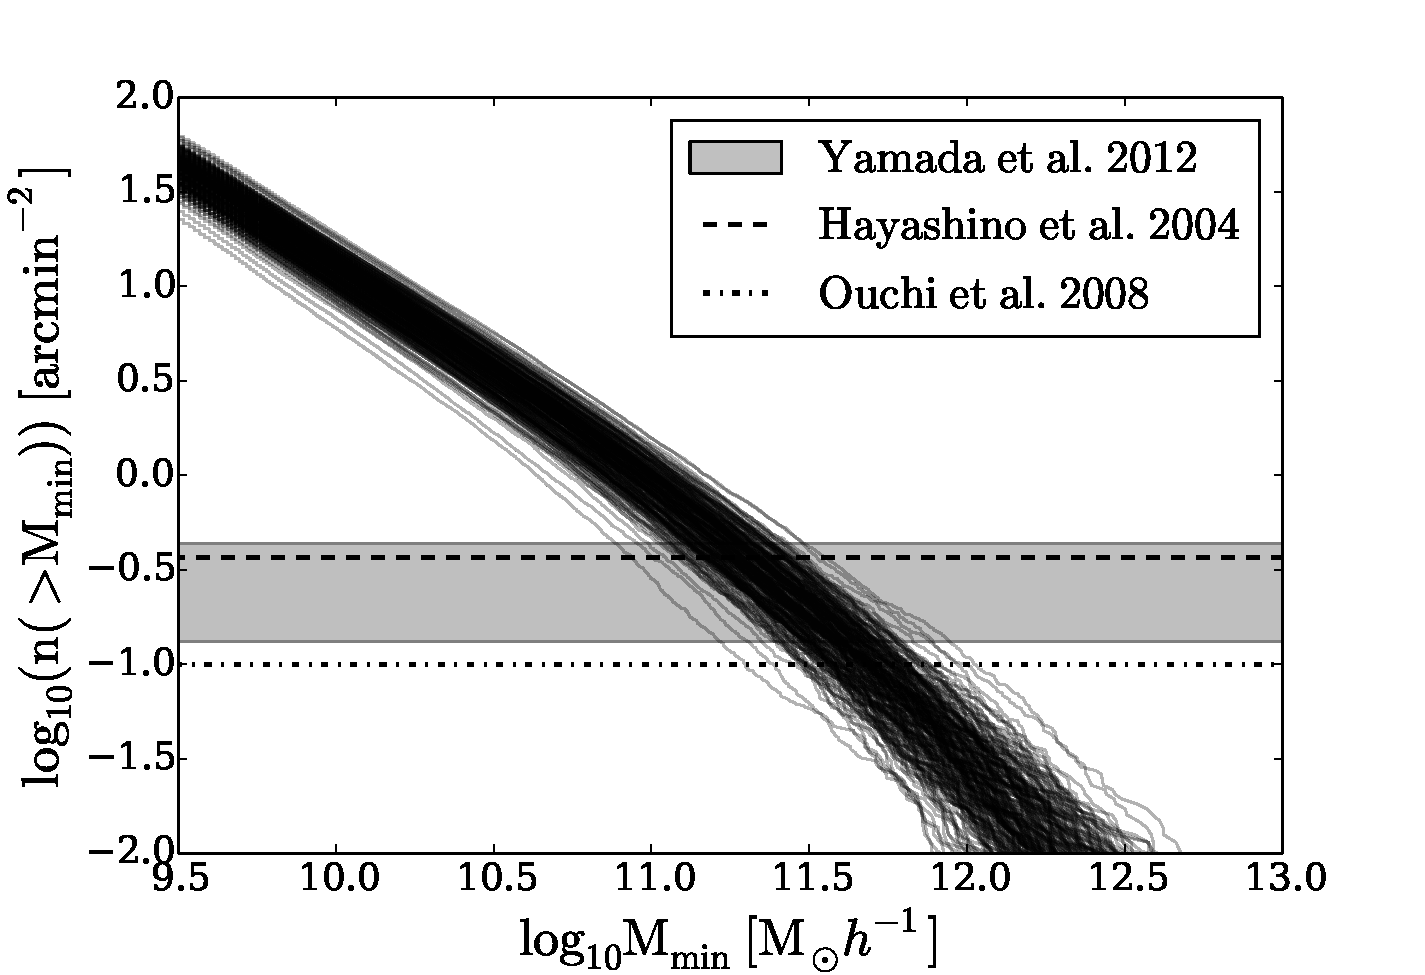
\includegraphics[width=0.45\linewidth,angle=0]{Fig1.pdf}
\caption{ \label{fig:halos} Left panel. Distribution of LAE number
  densities in all the fields observed by \citet{Yamada2012}. The
  point with the highest surface density corresponds to the densest
  sub-field in the SSA22 field. Right panel. Surface density of dark 
  matter halos as a function of a minimum halo mass to count the
  total number of elements in a volume. Each line represents one of the
  $210$ volumes of dimensions $46\times 35\times 41$ $h^{-3}$ Mpc$^{3}$
  in the Bolshoi simulation. The horizontal gray band represents the
  range of surface densities observed for LAEs at $z=3.1$ as reported
  by \citep{Yamada2012}.}
\end{center} 
\end{figure*}

The primary observational constraint we use in this paper is the LAE number
density information at $z=3.1$ obtained by the panoramic narrow-band
survey presented by \cite{Yamada2012} from a survey
conducted with the Subaru 8.2m telescope and the Subaru Prime Focus Camera,
which has a field of view covering $34\times 27$ arc-min, corresponding to a
comoving scale of $46\times35$ Mpc $h^{-1}$ at $z=3.09$.  The narrow
band filter used in the survey is centered at $4977$ \AA~with  $77$ \AA~width,
corresponding to the redshift range $z=3.062$-$3.125$ and $41$ \hMpc comoving scale for the detection of the Lyman-$\alpha$ line
centered at $z=3.09$. The authors reported a total  $2161$  LAEs with
an observed equivalent width, in the observer frame, larger than $190$
\AA~over a total survey area of $2.42$ deg$^{2}$ that includes 12
sub-fields,  this corresponds to average surface number density of
$0.24\pm 0.01$ arcmin$^{-2}$. 

The survey covered four independent fields:

\begin{enumerate}
\item The first is the SSA22
field of $1.38$ deg$^2$ with $1394$ detected LAEs (7 sub-fields), this
field has been known to harbor a region with a large density excess of
galaxies. 

\item The second observed region is composed by the fields Subaru/{\it
  XMM-Newton} Deep Survey (SXDS)-North, -Center and -South, with a
total of $0.58$ deg$^2$ and $386$ LAEs (3 sub-fields).

\item The third  field is the Subaru Deep Field (SDF) with $0.22$ deg$^2$ and
$196$ LAEs (1 sub-field), and 

\item The fourth one is the field around the Great Observatory
Optical Deep Survey  (GOODS-N) with $0.24$ deg$^2$ and $185$ LAEs (1
sub-field).  
\end{enumerate}
   

There is abundant observational work done on LAEs at redshift $z=3.1$
\citep{Kudritzki2000,Matsuda2005,Gawiser2007,Nilsson2007,Ouchi2008}.
However, we decide to focus on the data from \cite{Yamada2012} because
it has the largest covered area with homogeneous instrumentation
conditions (telescope, narrow band filter), data reduction pipeline
and conditions to construct the LAE catalog. This ensures that the
number density variations among fields are \emph{not} due to different
observational conditions or criteria to construct the catalogs.

{\bf A secondary benchmark is the angular correlation function
(ACF). \cite{Yamada2012} does not report an ACF measurement for
  their fields. Instead we use the results by   \cite{Ouchi2008} who
  reported the ACF is over a region of $1$ deg$^2$ over the SXDS
  field.  }

{\bf There are some differences between \cite{Ouchi2008} observations
  and those by \cite{Yamada2012}. The details in the color selection,
  corresponding limiting luminosities and EW thresholds are different
  in these references. In the case of
  \cite{Ouchi2008} the number density is $0.099\pm0.005$ arcmin$^{-2}$, which
  is 50\% lower that the median value of $0.20$ arcmin$^{-2}$ for the
  the general fields in \cite{Yamada2012}}



\subsection{The adequacy of including SSA22 as an observational benchmark}

{\bf The field SSA22 has been known to harbor a significant
  galaxy overdensity. \cite{Yamada2012} estimates that the densest
  sub-field is likely to be a rare density peak with $3-4\sigma$
  significance on the scale of $\sim 60$\hMpc. }

{\bf All the other sub-fields in SSA22 are average. They have a similar
  number density as other blank fields. The left panel in Figure
  \ref{fig:halos} shows the integrated distribution of LAEs number
  density in all the fields reported in  \cite{Yamada2012}. It is
  evident that there is only one sub-field  that stands out as an
  outlier in the distribution (it corresponds to  the densest field in
  SSA22). All the other fields form a continuous  distribution in
  number density.}   

{\bf Therefore, using the whole SSA22 region as a benchmark in the
  number density distribution does not impose any bias. However, on
  has to  keep in mind that is not plausible that the full number
  density distribution from a simulation will include a very dense
  field. We do not require the presence of such field to judge a mock
  distribution as successful. The statistical test we perform to
  compare mock distributions   against   observations does not require
  such a perfect match. }
  


\subsection{Simulation and halo catalogs}

The Bolshoi simulation \citep{Bolshoi} we use in this paper was
performed in a cubic volume of 250 $h^{-1}$ Mpc on a side. The
dark matter distribution is sampled using $2048^{3}$ particles, which
translates into a particle mass of $m_{\rm p}=1.35\times 10^{8}$
$h^{-1}$ M$_{\odot}$.  The cosmological parameters are consistent with
a WMAP5 and WMAP7 data with a matter density $\Omega_{\rm m} = 0.27$,
cosmological constant $\Omega_{\Lambda}=0.73$, dimensionless Hubble constant
$h=0.70$, slope of the power spectrum $n=0.95$ and normalization of the
power spectrum$\sigma_{8}=0.82$ \citep{Komatsu2009,Jarosik2011}.  

We use halo catalogs constructed with a Friend-of-Friends (FOF)
algorithm with a linking length of 0.17 times the inter-particle
distance. The catalogs were obtained from the publicly available
Multidark database \footnote{{\tt
    http://www.multidark.org/MultiDark/}}
\citep{MultiDark}. For each halo in the box we store its
comoving position in the box (3-D coordinates) and FOF mass. We focus our work
on halos more massive than $1\times 10^{10}$\hMsun that are resolved
with at least $70$ particles, the reasons for this choice are
explained in the next sub-section.  


\subsection{A model to populate halos with LAEs}
\label{subsec:mocks}



\begin{figure*}
\begin{center}
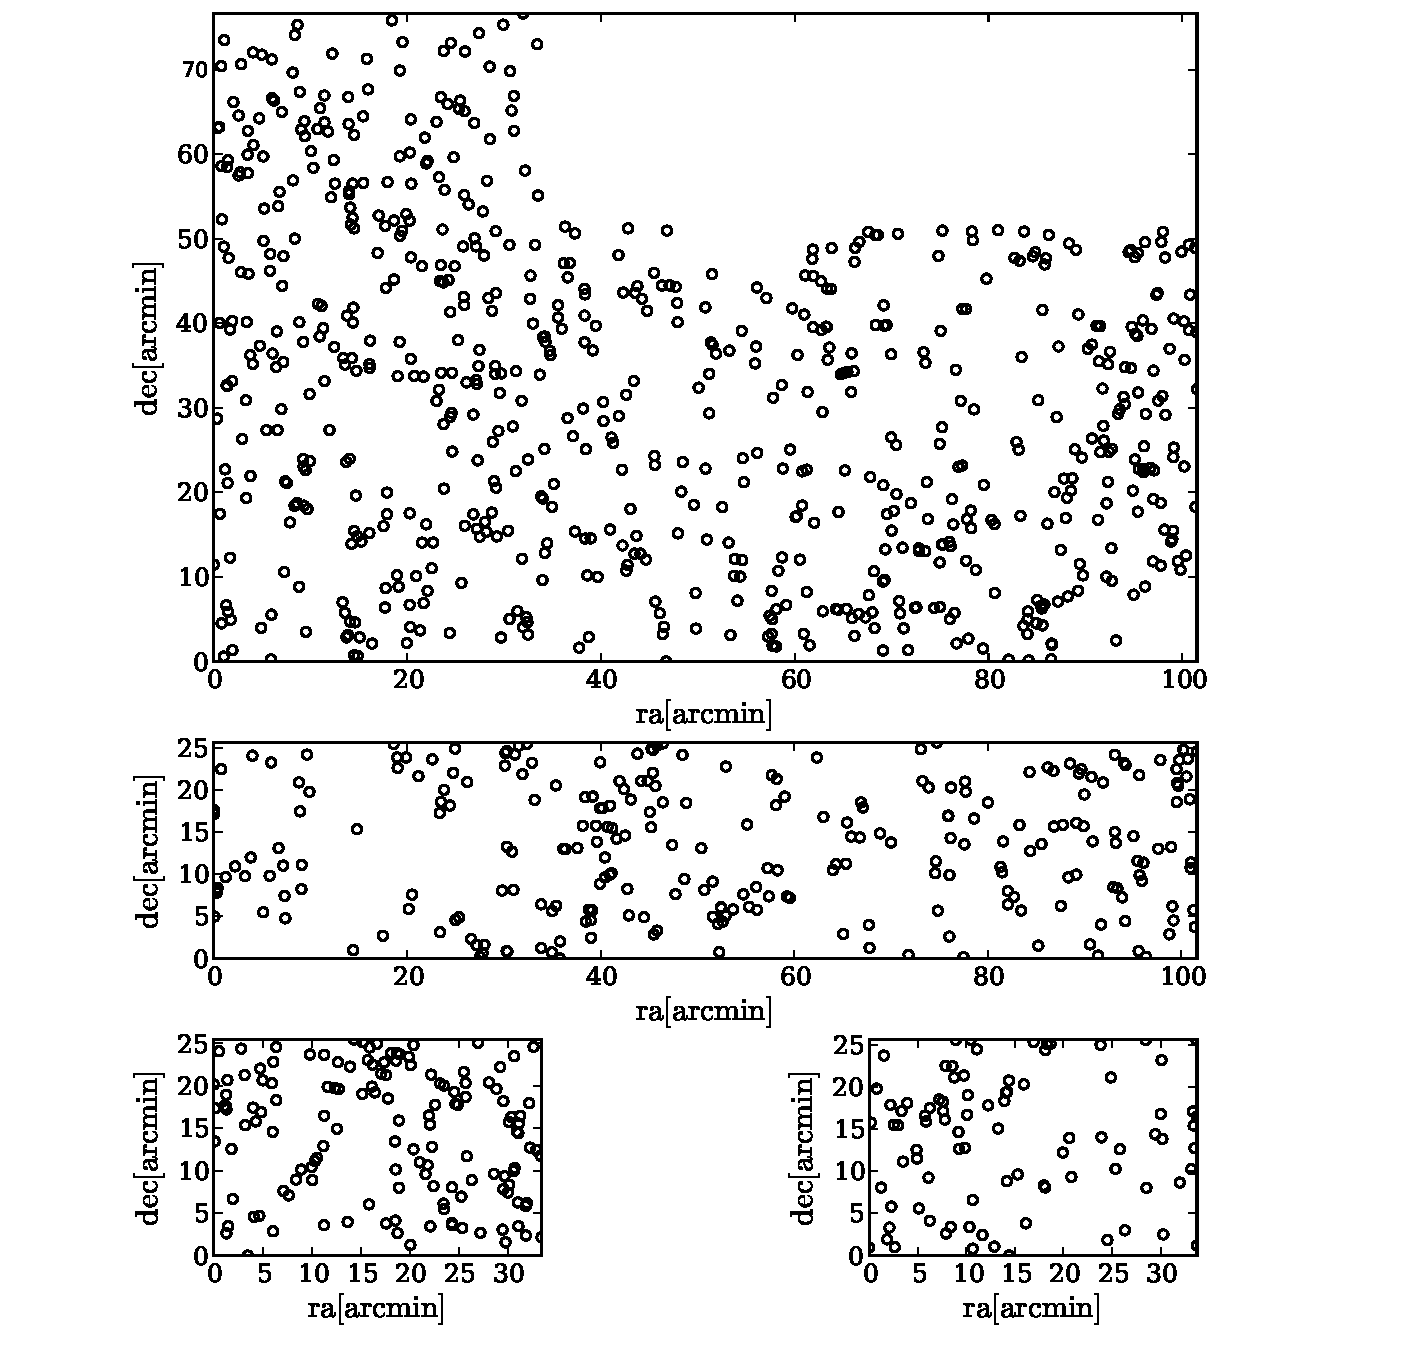
\includegraphics[width=0.8\linewidth,angle=0]{Figure0.pdf}
\caption{ \label{fig:distros} Spatial distribution of a LAEs mock
  survey for a model with parameters $\log_{10}M_{\rm min}=10.4$, $\log_{10}M_{\rm
    max}=10.5$ and $f_{\rm occ}=0.1$ for the {\texttt{match}}
  method. The larger panel shows $7$ mock
  fields together mimicking the SSA22 region. The intermediate panel
  shows $3$ mock fields corresponding to the SXDS region. The lower
  panels represent the SDF and GOODS-North fields. The same model has
  another 14 associated mock surveys build from different regions in
  the simulation, but constructed following the same pattern.}
\end{center} 
\end{figure*}


We assume that a dark matter halo can only host one
detectable LAE at most.  There are three parameters that
decide whether a halo host a LAE: the lower and upper bounds for the
mass range, $M_{\rm min}< M_{\rm h} < M_{\rm max}$, where LAEs reside and the fraction $f_{\rm occ}$ of such halos that host a detectable LAE. The reader
must keep in mind that the physical interpretation of the occupation
fraction $f_{\rm occ}$ convolves two phenomena: the actual presence of a star
forming galaxy in a halo and its detectability as a LAE.

{\bf We recall that we do not perform a explicit modeling for LAE
detectability. Our model does not assign a luminosity or escape
fraction for each LAE. We are interested in constraining the halo
mass range hosting detectable LAEs commonly used in photometric
narrow-band surveys. We also want to explore a wide range of
possible masses for the host halos without any strong theoretical
prejudice regarding the details of star formation in high-redshift
galaxies. }


In what follows we note by the letter ${\mathcal M}$ a model
defined by a particular choice of the three scalar parameters $M_{\rm
  min}$, $M_{\rm  max}$ and $f_{\rm occ}$. For each model ${\mathcal
  M}$ we create a set of mock fields from disjoint volumes in the
simulation. Each volume has the same geometry probed by Suprime-CAM
and the narrow band filter, namely rectangular cuboids of dimensions
$46\times 35\times 41$ $h^{-3}$ Mpc$^{3}$ where the last dimension goes
in the redshift direction. This corresponds to a total area of $880$
arcmin$^{2}$ in each mock field. We construct a total $5\times 7
\times 6=210$ of such volumes from a snapshot in the Bolshoi
simulation. In each mock field a LAE is assigned to the position of a
dark matter halo if the halo mass is in the range allowed by the model
$M_{\rm min}<M_{\rm h}<M_{\rm max}$ and a random variable taken from
an homogeneous distribution $0\leq \xi<1$ is smaller than the occupation
fraction $\xi<f_{\rm occ}$.

Next we construct mock surveys by making groups of $12$ mock fields
out of the $210$ available volumes. In total $15$ mock surveys are
constructed for each model $\mathcal{M}$. The grouping of the $12$
mock fields into a mock catalog is done in two different ways. The
first is called {\texttt{match}}, it follows the clustering of the
observational fields. From the $12$ mock fields, $7$ are constructed
from contiguous fields in the simulation to mimic the SSA22 region,
$3$ are also contiguous between them but not to the first $7$ fields
to mimic the SXDS fields and finally $2$ non-contiguous fields to
imitate the SDF and GOODS-North field.   The second way to group the
mock fields is called {\texttt{random}}, whereby all the $12$ fields
are selected in such a way as to avoid that any two volumes are
contiguous. In this \documentname we only report the results obtained
by the {\texttt{match}} method and mention explicitly differences
observed with the {\texttt{random}} selection. 

Figure \ref{fig:distros} shows the spatial distribution for one mock
survey constructed using the {\texttt{match}} method. Each field
corresponds to one of the observational fields. The model parameters
to build the mock are $M_{\rm min}=10^{10.4}$\hMsun, $M_{\rm
  max}=10^{0.5}$\hMsun and $f_{\rm occ}=0.1$. The figure shows only
one out of the $15$ different mock surveys that are constructed for
each model. We note that we only use $15\times 12=180$ mock fields out of the
total of $210$ available sub-volumes. The reason is that the {\texttt{match}}
method imposes constraints on the way the $7$ fields mimicking the
SSA22 can be distributed. This restriction makes unable some of the
sub-volumes in the box. We decide to keep the number of mock surveys
fixed to $15$ also for the {\texttt{random}} method in order to allow a
fair comparison between the two methods.

\subsection{Exploring and selecting good models}

We make a thorough exploration of the parameter space for the models
${\mathcal M}$ where $\log_{10} M_{\rm min}$ takes $30$ values from $10.0$ up
to $12.9$ with an even spacing of $0.1$ dex. $\log_{10} M_{\rm max}$
takes values in the same range as $\log_{10}M_{\rm min}$ only with a
displacement of $0.1$ dex in the whole range. The occupation fraction
$f_{\rm occ}$ takes $10$ different values from $0.1$ to $1$ regularly
spaced by $0.1$. In total the number of different models ${\mathcal
  M}$ that are explored is $30 \times 30 \times 10 = 9000$.  

The lower limit for the parameter $M_{\rm min}$ is set by the minimum
occupation fraction we decide to consider. At $M_{\rm
  min}=10^{10}$\hMsun the halo number density around that mass range
is $\sim 10$ times higher than the observational constraints
for LAEs. This means that models in that mass range and an occupation fraction $f_{\rm  occ}=0.1$ have the possibility to be compatible with
observations. Lower values for $M_{\rm min}$ require $f_{\rm
  occ}<0.1$, which are not considered in this \documentname.  {\bf In
  turn exploring occupation fractions on the order of $f_{\rm occ}=0.01$ 
  only makes sense for halo populations in the mass range of
  $10^{9}$\hMsun which are abundant enough to fit observations with a
  very low occupation fraction. In our case, this is a mass range unresolved
  by the Bolshoi simulation and therefore cannot be considered in the
  present study.}


For each mock survey generated in a given model ${\mathcal M}$ we
compute the surface density in its $12$ mock fields. We perform a
Kolmogorov-Smirnov (KS) to compare these values against the $12$
observational values. This tests gives us a value $0<P<1$ to
reject the null hypothesis, namely that two data sets come from the
same distribution. In this paper we consider that for values $P>0.05$
the two distributions can be thought as coming from the same
distribution.

We begin by considering that  a model ${\mathcal M}$ with at least one
mock survey (out of 15) consistent with observations has viable
parameters to host LAEs. From that we consider a stronger constraints
to reduce the number of models by asking that all the 15 mocks to be
consistent with observations and analyze again the properties of the
resulting models. Finally we add the ACF as an additional constraint
and consider all the models having their $15$ mocks consistent with
observations. 

{\bf The ACF is computed using  the Landy \&  Szalay estimator
  \citep{Landy1993}  on fields of size $1$ deg$^2$ to be compared
  against the results reported by \cite{Ouchi2010}.}

The observed and mock ACF are fit to a power-law function:
\begin{equation}
\omega(\theta) = \left(\frac{\theta}{\theta_{0}}\right)^{-\beta}, 
\label{eq:fitting}
\end{equation}
where $\theta_0$ and $\beta$ are free parameters. The fit is done
using a least square minimization procedure. For each mock field we
obtain a covariance matrix that gives us the uncertainty in the
parameters $\beta$ and $\theta_0$. {\bf We consider that a mock field is
consistent with observations if the two parameters $\beta$ and
$\theta_0$ are equal within a $1$-$\sigma$ range.}
 
\section{Results}
\label{sec:results}

\begin{figure*}
\begin{center}
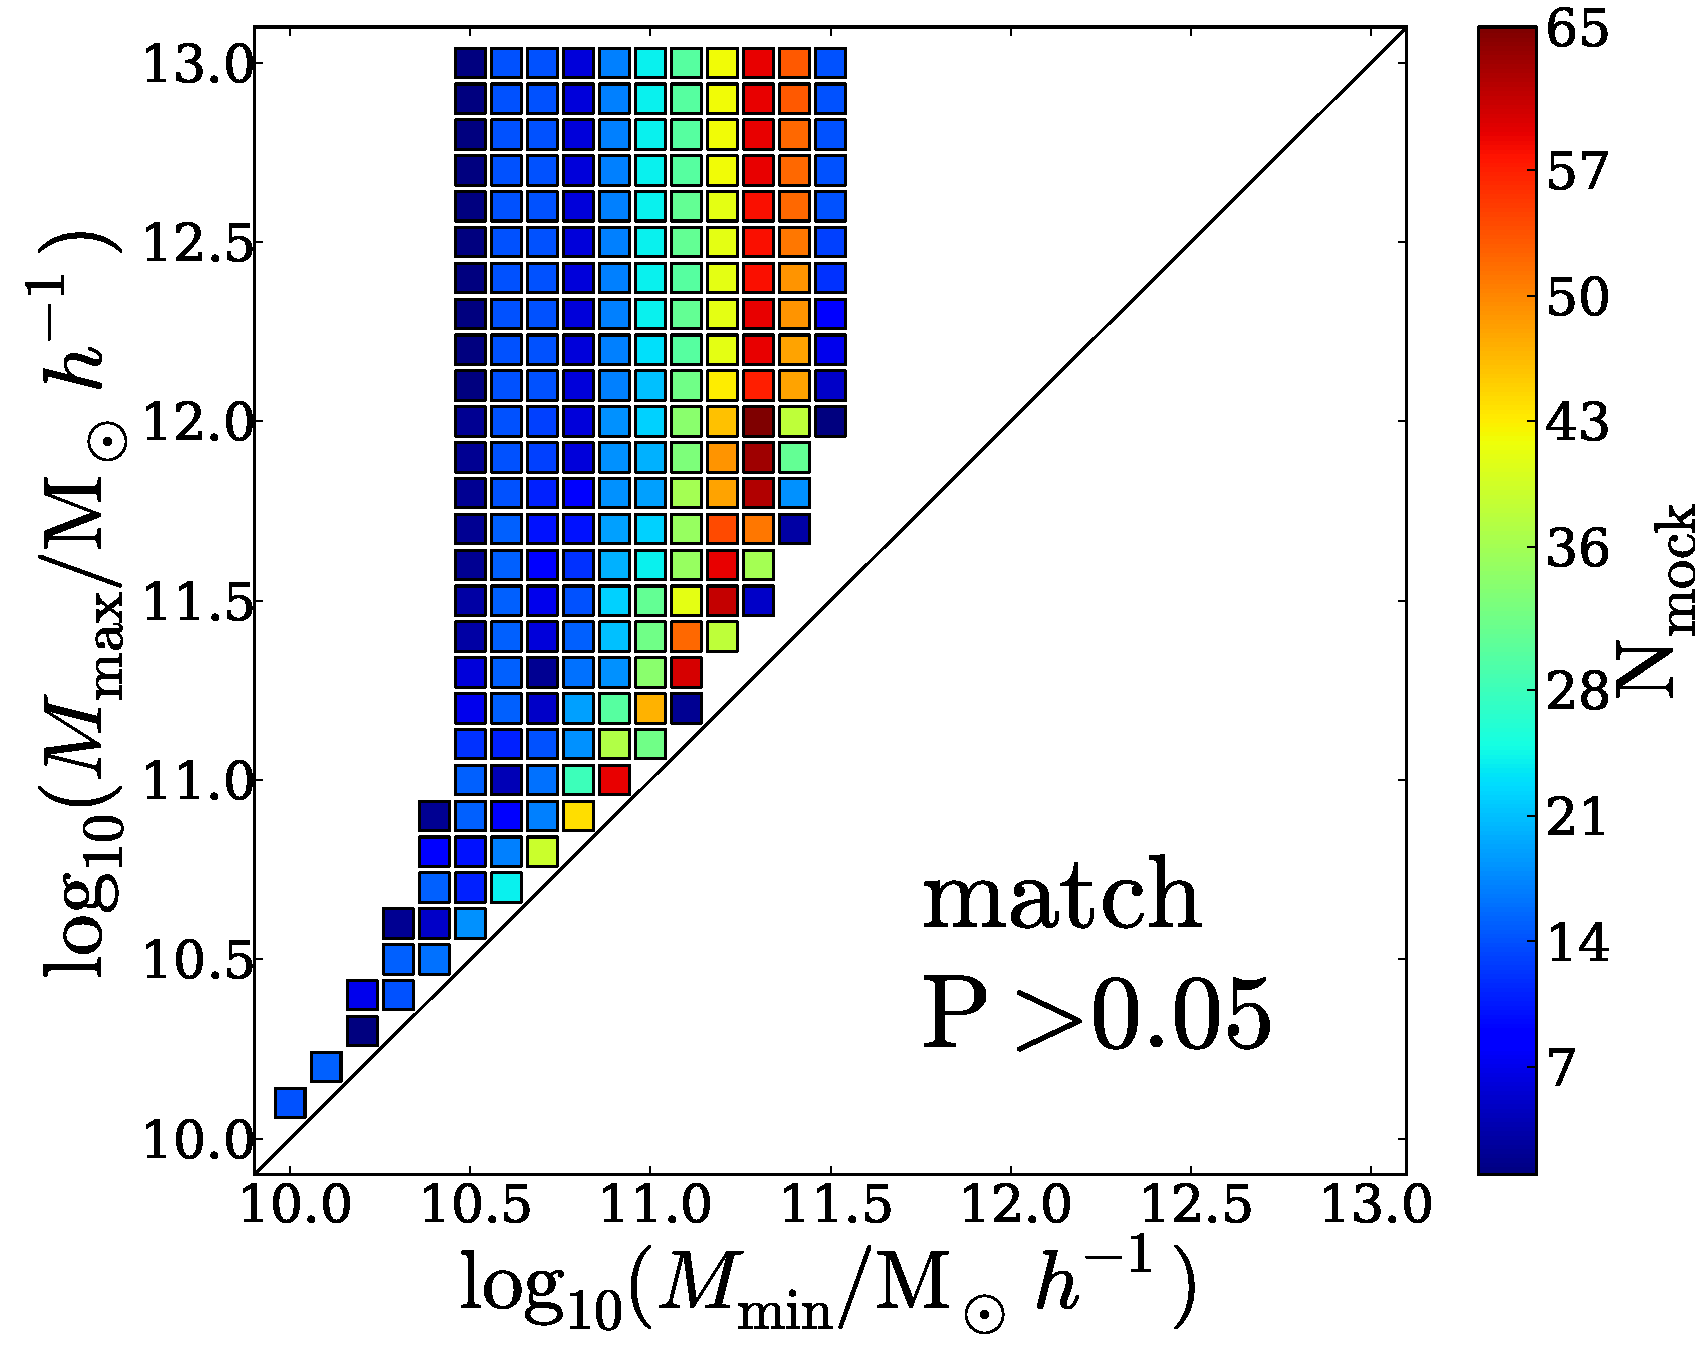
\includegraphics[width=0.46\linewidth,angle=0]{Fig2_match_P5.pdf}
\vspace{5mm}
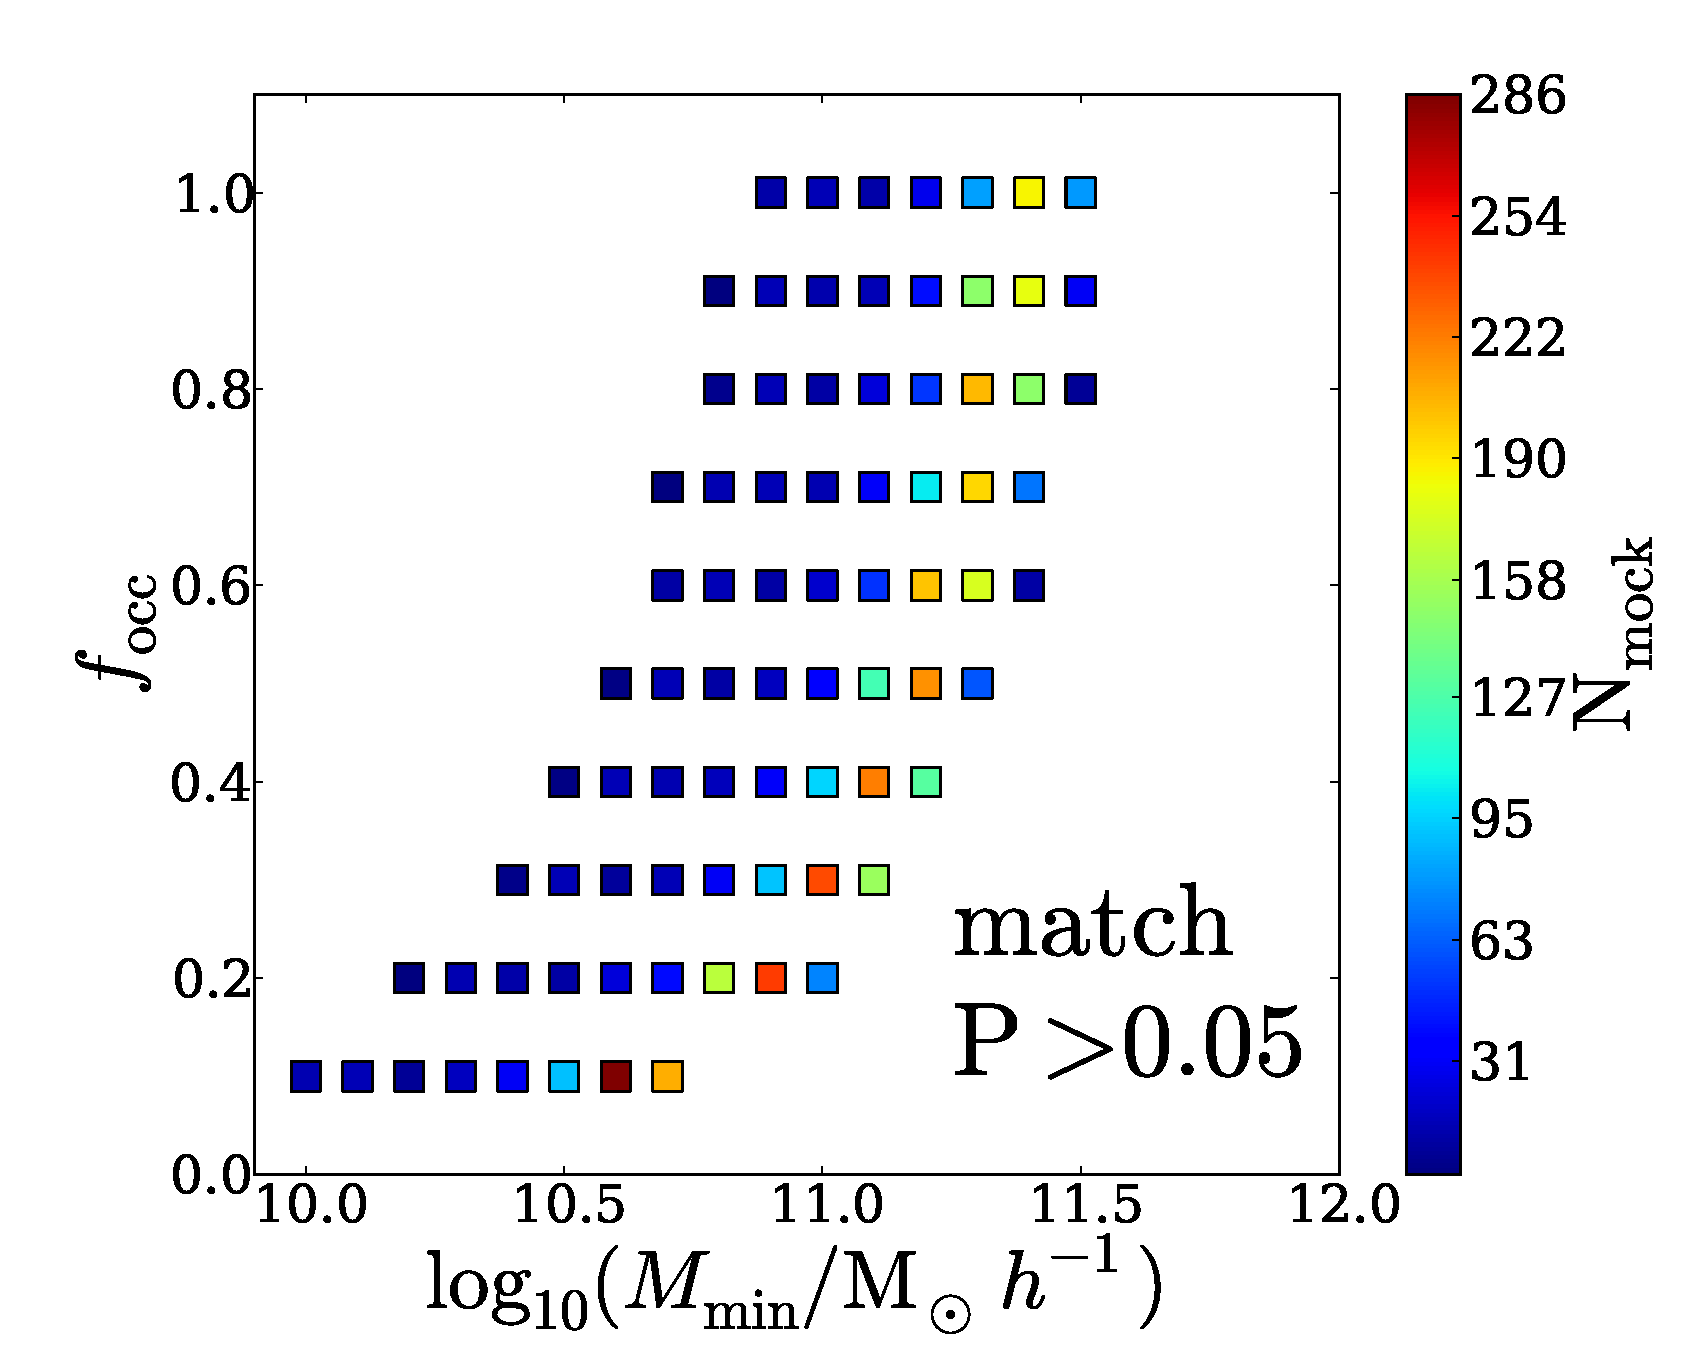
\includegraphics[width=0.49\linewidth,angle=0]{Fig3_match_P5.pdf}
\end{center} 
\caption{$M_{\rm min}$-$M_{\rm max}$ (left) and $M_{\rm    min}$-$f_{\rm
    occ}$ (right) planes for all models with  KS test values
  $P>0.05$. The color code corresponds to the number of mock surveys
  compatible with observations. Only regions of parameter  space with
  at least one consistent mock survey are
  included. \label{fig:landscape}}      
\end{figure*} 

The main purpose of this section is to show how different
observational constraints narrow down the parameters space of allowed
models. Each sub-section presents the effect of adding a new piece of 
observational or statistical evidence. 


\subsection{Dark Matter Halo Number Density}

The right panel in Figure \ref{fig:halos} shows the  integrated dark matter halo surface
density as a function of  minimum halo mass $M_{\rm min}$. Each line
corresponds to one of the 210 sub-volumes in the Bolshoi
simulation. The gray band indicates the surface density values for
LAEs allowed by observations \citep{Yamada2012}. The dashed lines
represent the average values in the fields observed by
\citep{Ouchi2008}. 
 
This plot allows us to understand why only a specific range of
models ${\mathcal M}$ can be expected to be consistent with
observations. From Figure \ref{fig:halos} we can read that models with
a minimum mass $M_{\rm min}>10^{12}$\hMsun always have a
surface number density lower than the observational constrain, making
them incompatible with observations; there are simply too few halos compared to observed
LAEs. The opposite is true in models with $M_{\rm
  min}<10^{11.0}$\hMsun that have a surface number density larger
observations. In those cases the maximum mass $M_{\rm max}$ and the
occupation fraction $f_{\rm occ}<1.0$  can be tuned in order to lower
the halo number density to match observations.   


Figure \ref{fig:halos} also illustrates the impact of cosmic
variance. At fixed minimum mass there is an scatter of $0.3-0.6$ dex
in the number density abundance, which is of the same order of
magnitude as the scatter in the observational data.  As a consequence, the variation in
the number density in mocks for models with the same mass range and occupation
fraction can be by factors of $\sim 2-5$.  This scatter induced by
cosmic variance is naturally included in the mock construction
process. This variance will explain that very different models can be
made compatible with observations. 


\subsection{Models consistent with the surface density distributions}


Figure \ref{fig:landscape} presents regions in parameter space $M_{\rm
min}$-$M_{\rm max}$, $M_{\rm min}$-$f_{\rm occ}$ where the KS test
between the mocks and observations yields values of $P>0.05$ for at
least one mock survey in each model. For those models it
is not possible reject the hypothesis that the simulated and observed
data for the surface number density come from the same parent
distribution. 

In total, there are between $550$ to $600$ models out of the original
$9000$ models that have at least one mock survey consistent with
observations. By inspection of Figure \ref{fig:landscape} we see that
the halo number abundance is able to constraint the minimum mass
$M_{\rm min}$ to a narrow range, while $M_{\rm max}$ and $f_{\rm occ}$
remain largely unconstrained. 

In Figure \ref{fig:landscape} there are three regions of parameter
space that can be clearly distinguished. The first corresponds to
models where the minimum mass is high $M_{\rm min}>
10^{11.5}\hMsun$.  For these models the number density of LAEs is too low
to be compatible with observations. 

The second region corresponds to an intermediate range for the minimum
mass $10^{10.5}\hMsun < M_{\rm min}< 10^{11.5}\hMsun$ where,
regardless of the value of the maximum mass $M_{\rm max}$, it is
possible to tune the occupation fraction $f_{\rm occ}$ to bring some
of the mock surveys into good agreement with observations. In this
region we find two extreme kinds of models. One extreme are models
with a narrow mass interval $\Delta M\equiv \log_{10} M_{\rm max}
- \log_{10}M_{\rm  min} <1.0$ dex. The other extreme are models with a
large mass interval $\Delta M>1.0$ dex going up to the maximum halo
mass present in the simulation at that redshift, with $\Delta M = 2.5$
dex in some cases. 
  
The third region in parameter space corresponds to $M_{\rm
  min}<10^{10.5}\hMsun$. In this case only models with a very narrow
mass interval of at most $0.5$ dex ($M_{\rm max}<10^{11.0}\hMsun$) and low
occupation fractions $f_{\rm occ}\leq 0.3$ are allowed. 

Without any additional information our method allows us to infer that
most of the successful models are found in the second and third regions of
parameter space. This result was expected from halo
abundance calculations shown in Figure \ref{fig:halos} and discussed
in the previous subsection. 

However, the additional information we gain with this test is the
relative abundance of models in the parameter space. Not all 
models in the second region have an equal abundance. By inspection of
Figure \ref{fig:landscape} it seems that models with $\log_{10}M_{\rm
  min}\sim 10^{11.3}$\hMsun and low occupation fraction $f_{\rm}\leq 0.3$
are preferred.  In the next sub-sections we explore in detail the
models in this region, imposing tighter constraints on the KS test
results and exploring the mocks' consistency with the angular correlation
function.  

 
\subsection{Models with the largest number of consistent mock surveys}


\begin{figure*}
\begin{center}
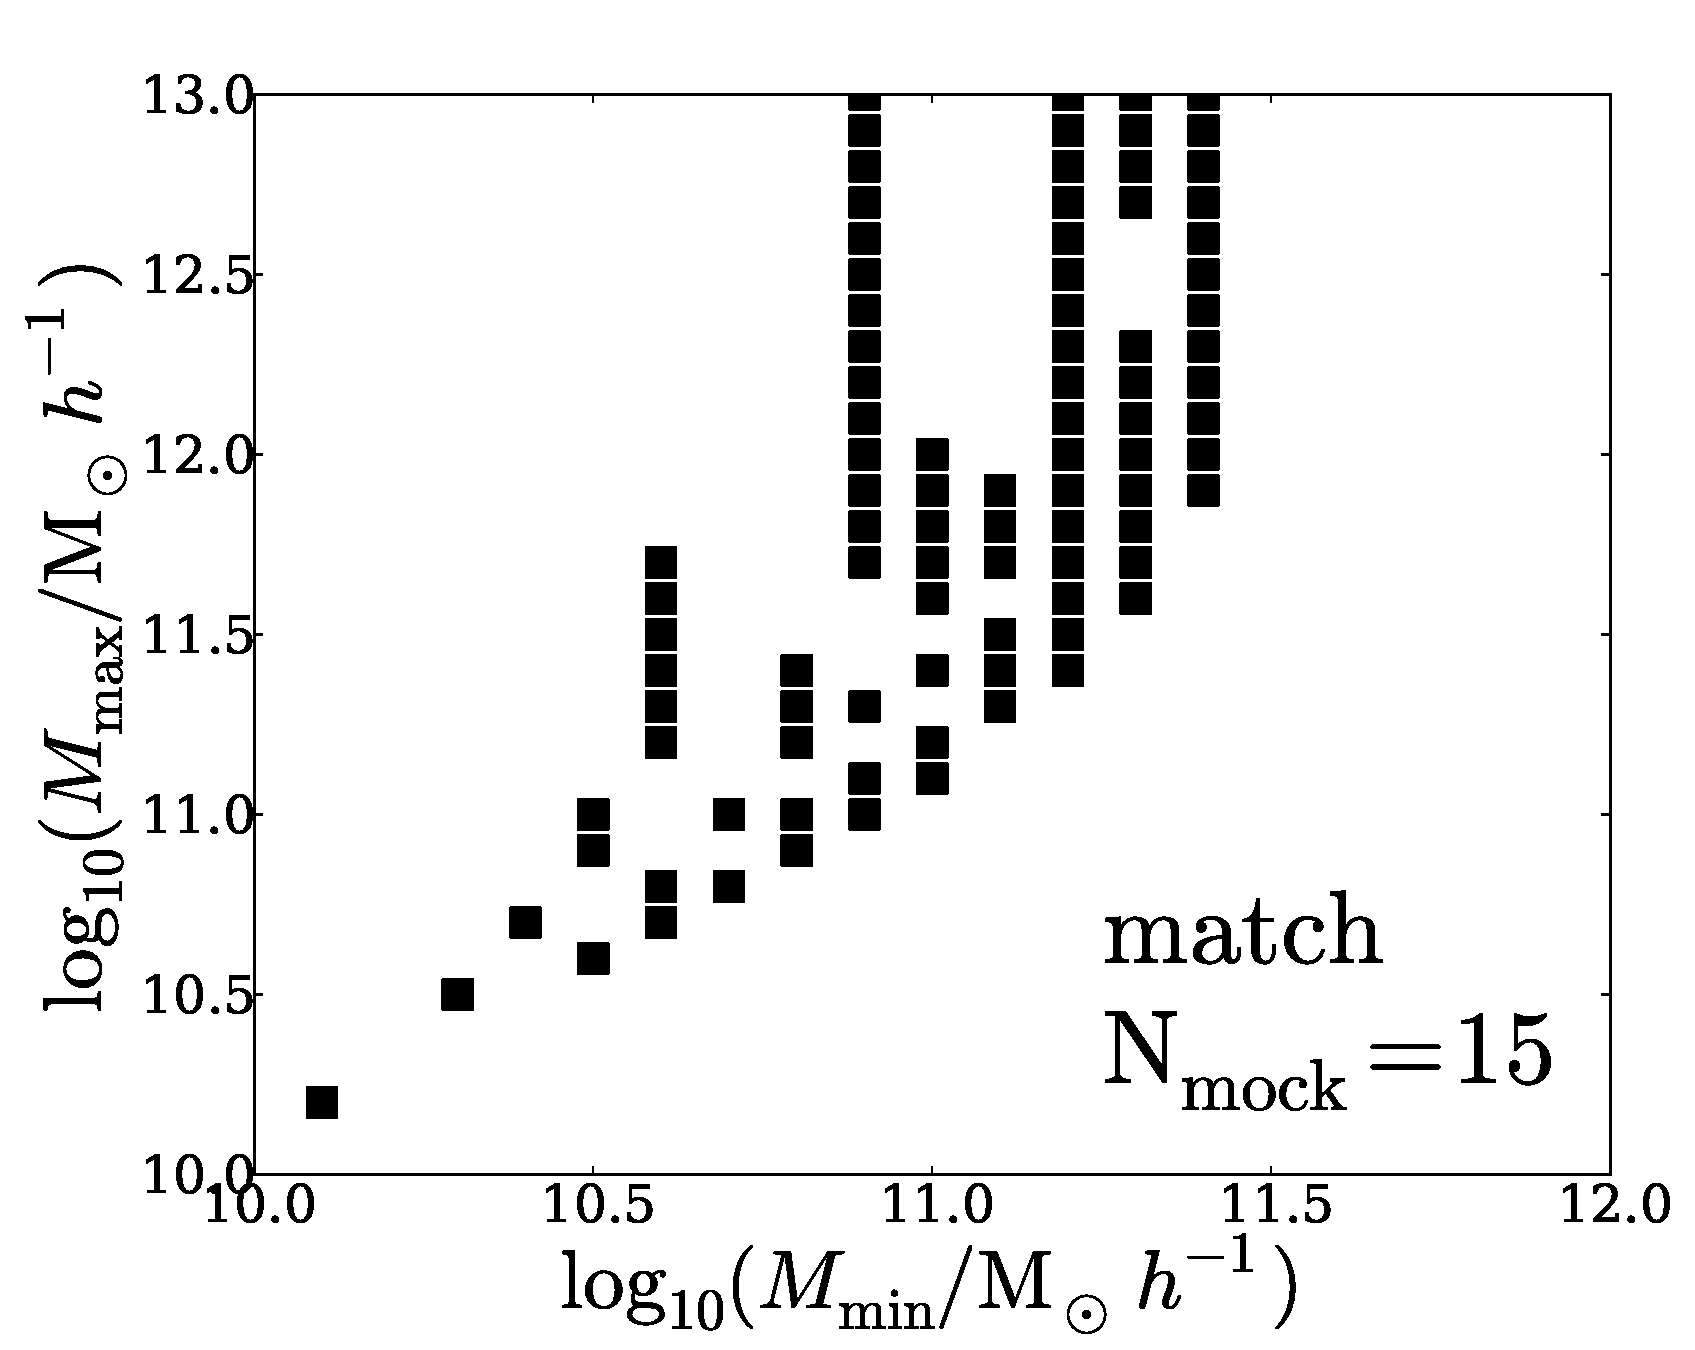
\includegraphics[width=0.46\linewidth,angle=0]{Fig5_match_mass_mock.pdf} 
\hspace{5mm}
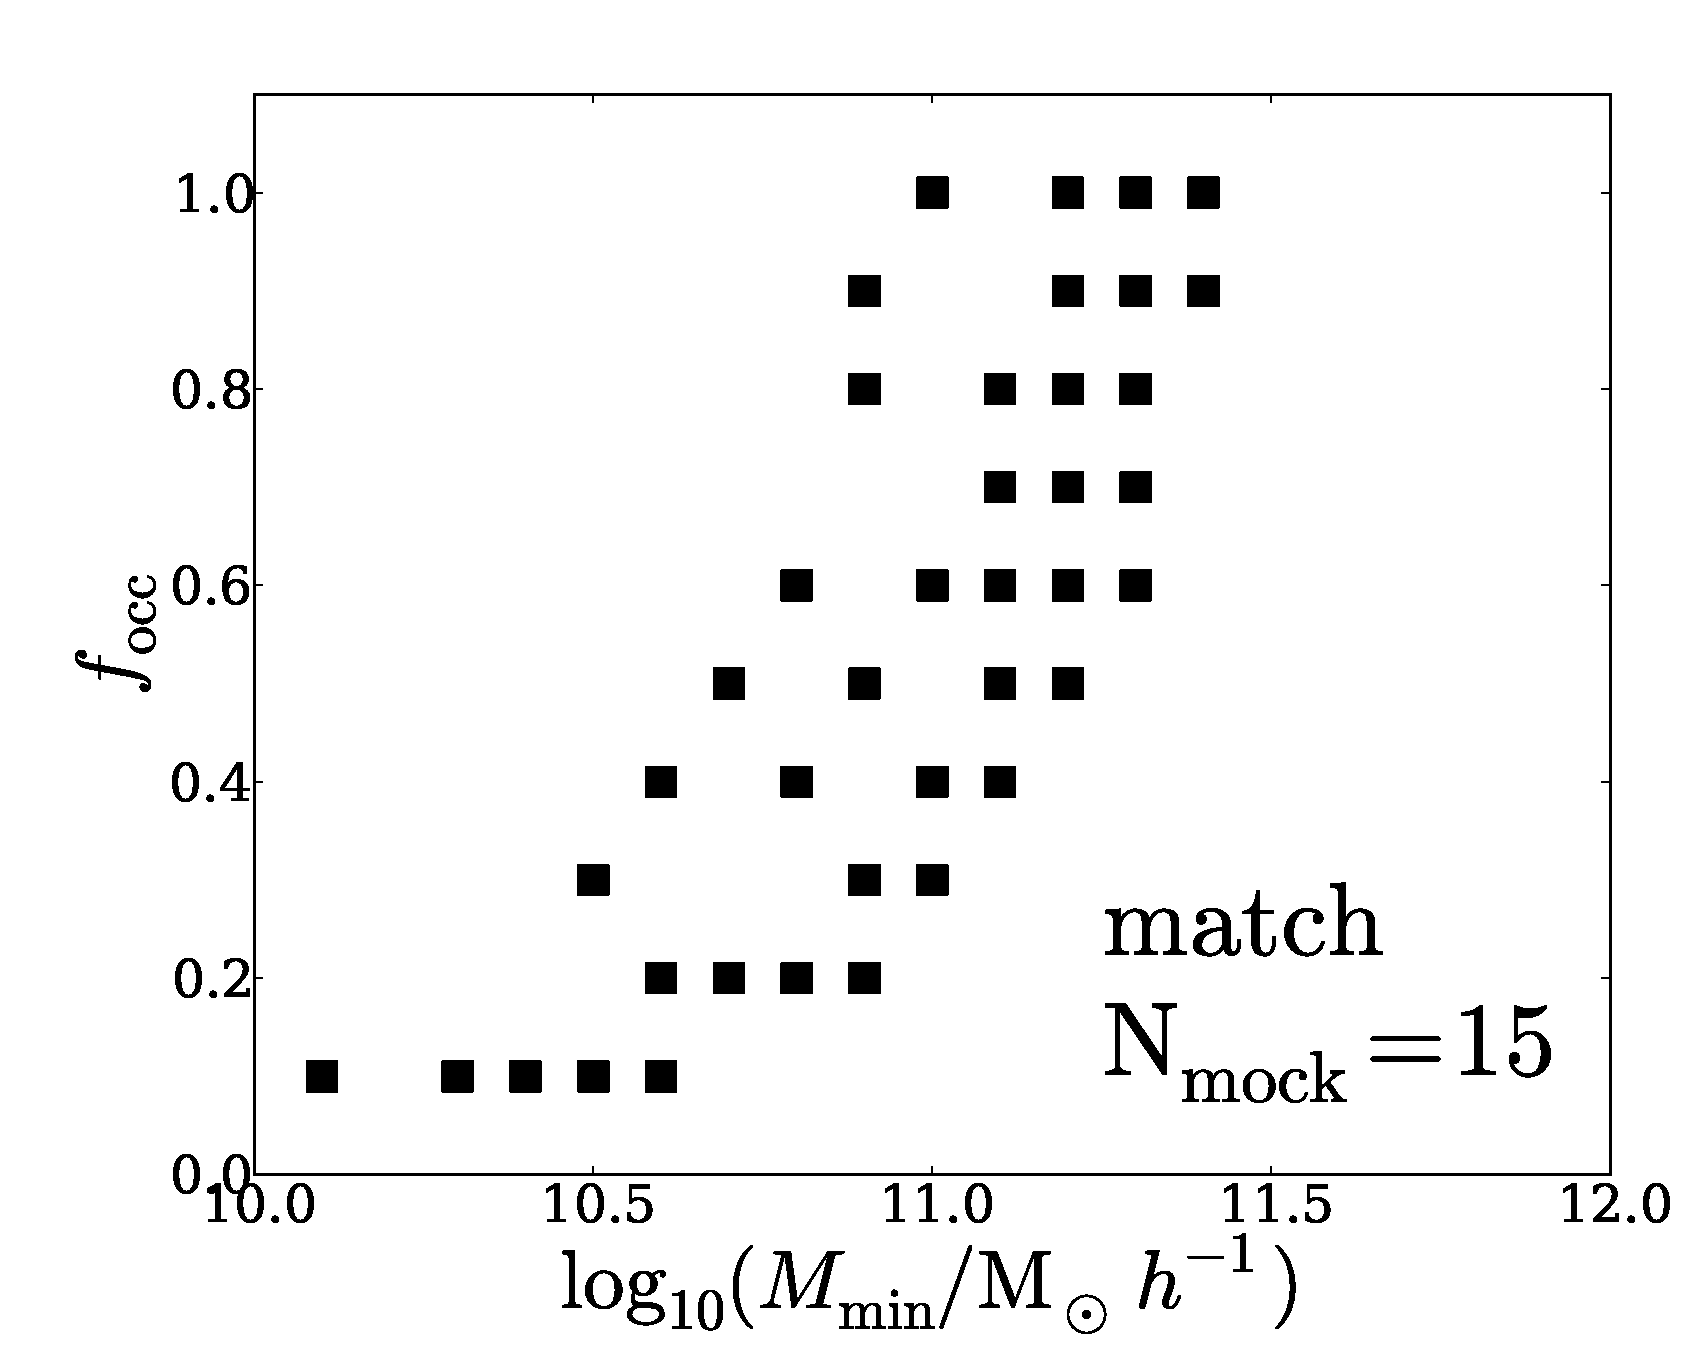
\includegraphics[width=0.46\linewidth,angle=0]{Fig5_match_f_occ_mock.pdf}
\end{center}  
\caption{Favored regions in parameter space when the constraints on
  the maximal number of consistent mocks is imposed. Only the results
  for the {\texttt{match}} method are shown.
  \label{fig:restriction_mock}}  
\end{figure*}


In the previous sub-section we use a conservative criterion of
agreement by selecting the models that had at least one mock survey
with $P>0.05$ in the KS test. Now we turn to a more strict selection
by requiring all the 15 constructed mock surveys to be consistent with
observations. 


With this cut we find $\sim 100$ models with all the 15 mock survey
realizations with $P>0.05$.  This cut represents a reduction by a
factor of $\sim 6$ with respect to the total number of models with at
least one consistent mock.

Figure \ref{fig:restriction_mock} presents the locii of these models
in the parameter space $M_{\rm min}-M_{\rm max}$ and $M_{\rm
  min}-f_{\rm occ}$. With this constraint the number of consistent
models with  $10.5 < \log_{10}M_{\rm min}< 11.0$ are reduced. This 
corresponds to the regions in the parameter space in
Figure \ref{fig:landscape} that already had a low number of 
consistent mock surveys. On the other hand, from the right panel in
Figure \ref{fig:restriction_mock} we see that the favored occupation
fraction  still remain unconstrained $0\leq f_{\rm  occ}\leq 1.0$. 

We conclude that conditions on the number density statistics, even if they are
very strict, only put strong constraints on the minimum mass $M_{\rm
  min}$ but not on the other two parameter of the model $M_{\rm max}$
and $f_{\rm occ}$. 



\subsection{Consistency with the Angular Correlation Function}



Figure \ref{fig:correlation_parameters} shows the results for the
best estimates of $\theta_{0}$-$\beta$  used in the ACF
parameterization.  Blue circles with error bars represent the results
from the mocks and the horizontal line the observational results of
\cite{Ouchi2010} over a field with average number density where the
$\beta$ parameter was fixed in the fit. From this Figure we observe
that there are models with too large values of $\theta_0$ and $\beta$
that can be ruled out as inconsistent with the angular correlation
function. 

Figure \ref{fig:restriction_mock_and_f_occ_corr} presents the
remaining consistent models in the planes $M_{\rm min}$-$M_{\rm
  max}$ and $M_{\rm   min}$-$f_{\rm occ}$. A model is consistent with
observations if there is a $1$-$\sigma$ overlap between both the
correlation length $\theta_0$ and the exponent $\beta$.  We find that
we end up with $40$ models consistent with the ACF constraints.  

Comparing Figure
\ref{fig:restriction_mock_and_f_occ_corr} with Figure
\ref{fig:restriction_mock} we see that the new constraint disfavors
almost all models with $M_{\rm max}>10^{12}$. The only exception is 
a narrow range of models with $M_{\rm min}=10^{10.9}$. However, we
have verified that these models are only marginally consistent with
the ACF constraints in the $\theta_0$-$\beta$ plane.

From this comparison we conclude that clustering information can
constraint the values of $M_{\rm max}$, but not the occupation
fraction. 


\begin{figure}
\begin{center}
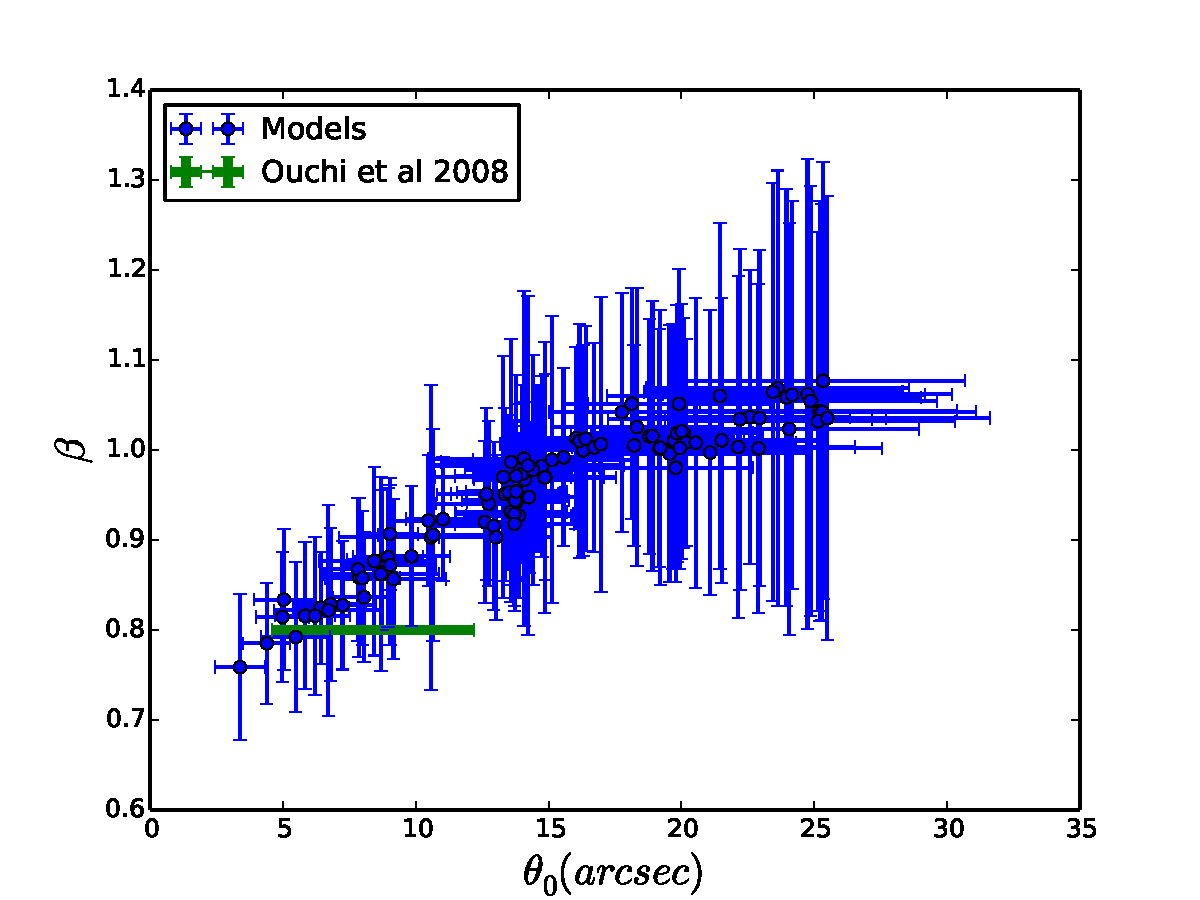
\includegraphics[width=1.0\linewidth,angle=0]{power_law_correlation_degree2.pdf}  
\end{center}
\caption{Values for the free parameters $\theta_{0}$ and $\beta$
in the fitting formula (Eq. \ref{eq:fitting}) for the angular
correlation function. Blue dots correspond to simulations and the
green line to observations by \citet{Ouchi2010}. The error
bars in the theoretical data correspond to the quadratic average of
the fitting errors for each mock
survey \label{fig:correlation_parameters}} 
\end{figure} 


\section{Discussion}
\label{sec:discussion}

\begin{figure*}
\begin{center}
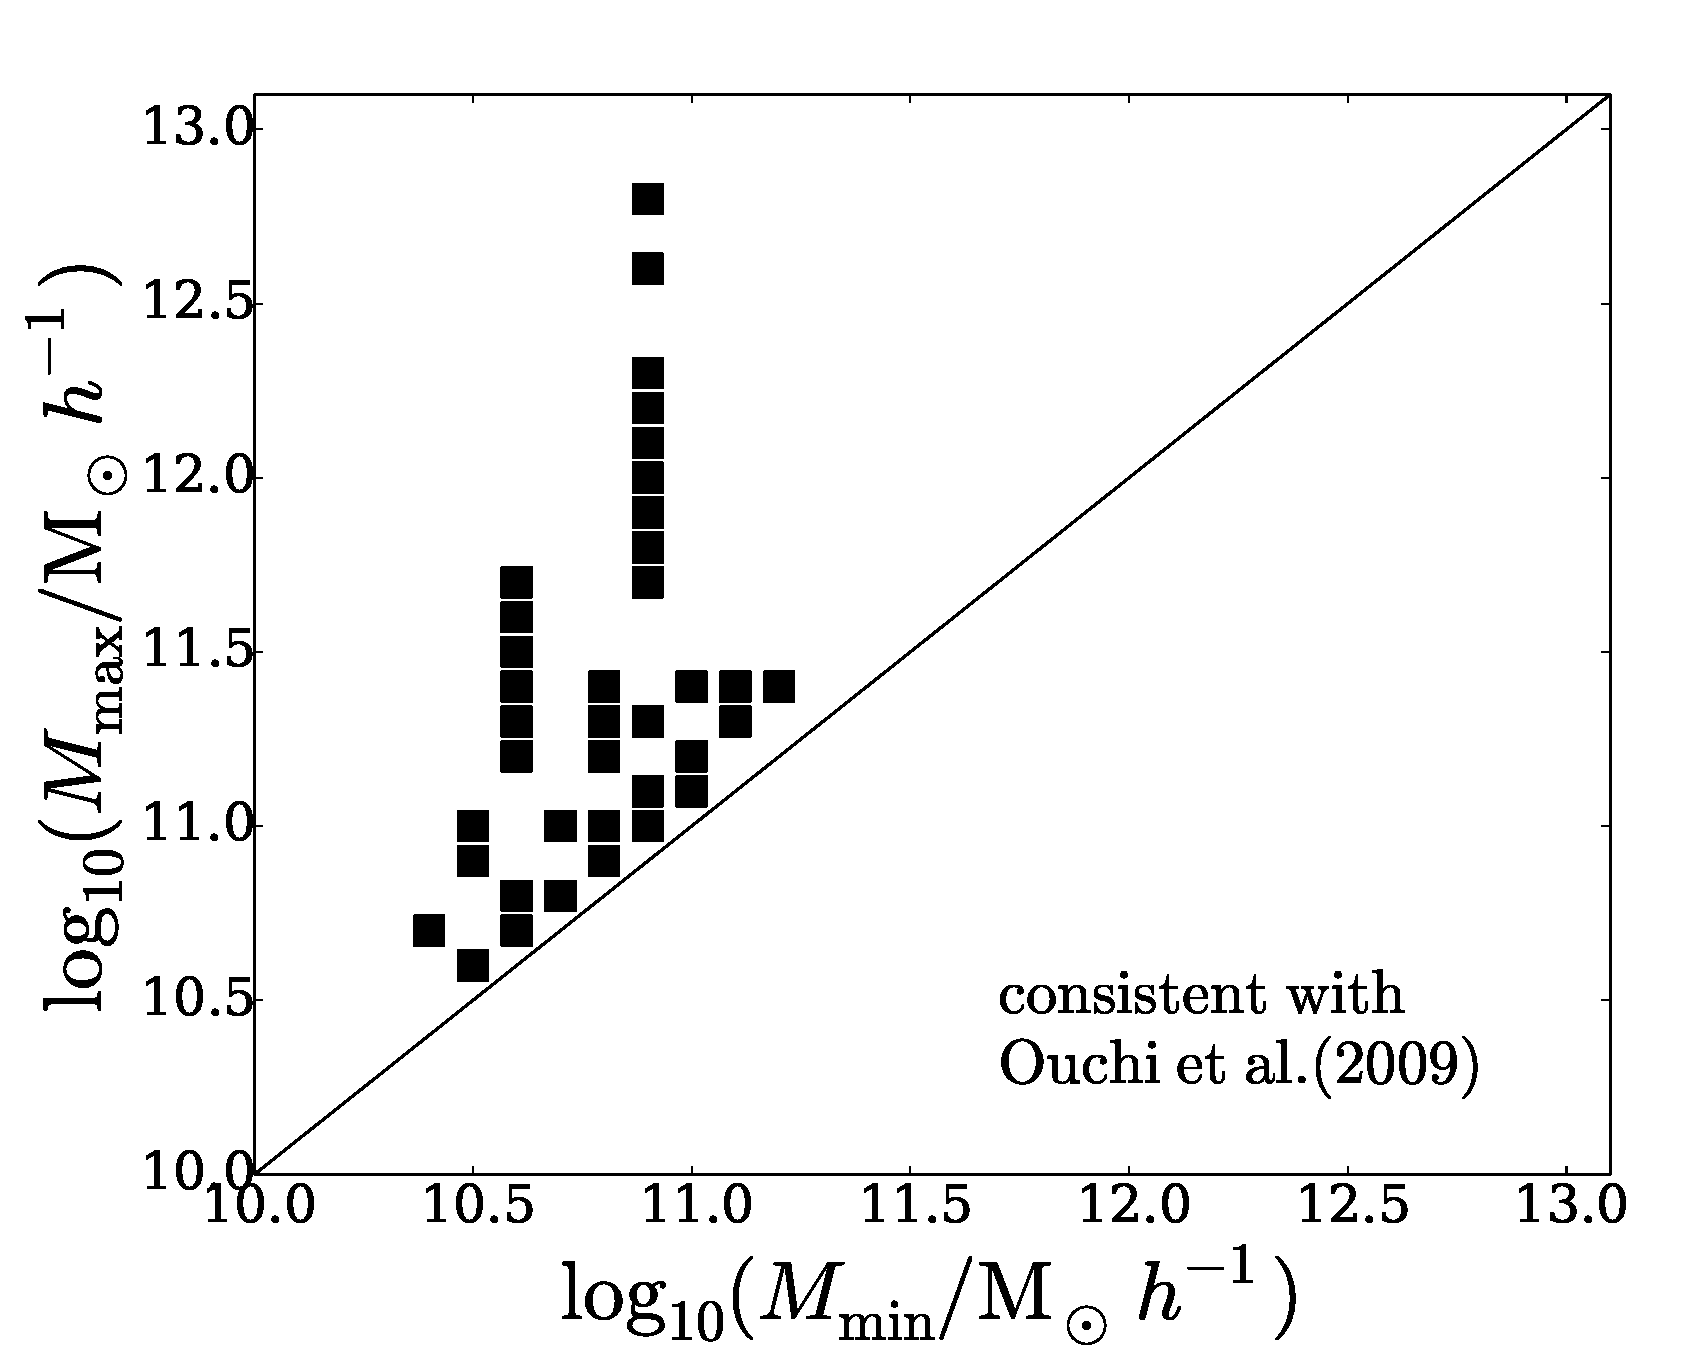
\includegraphics[width=0.46\linewidth,angle=0]{Fig6_mass.pdf}
\hspace{5mm}
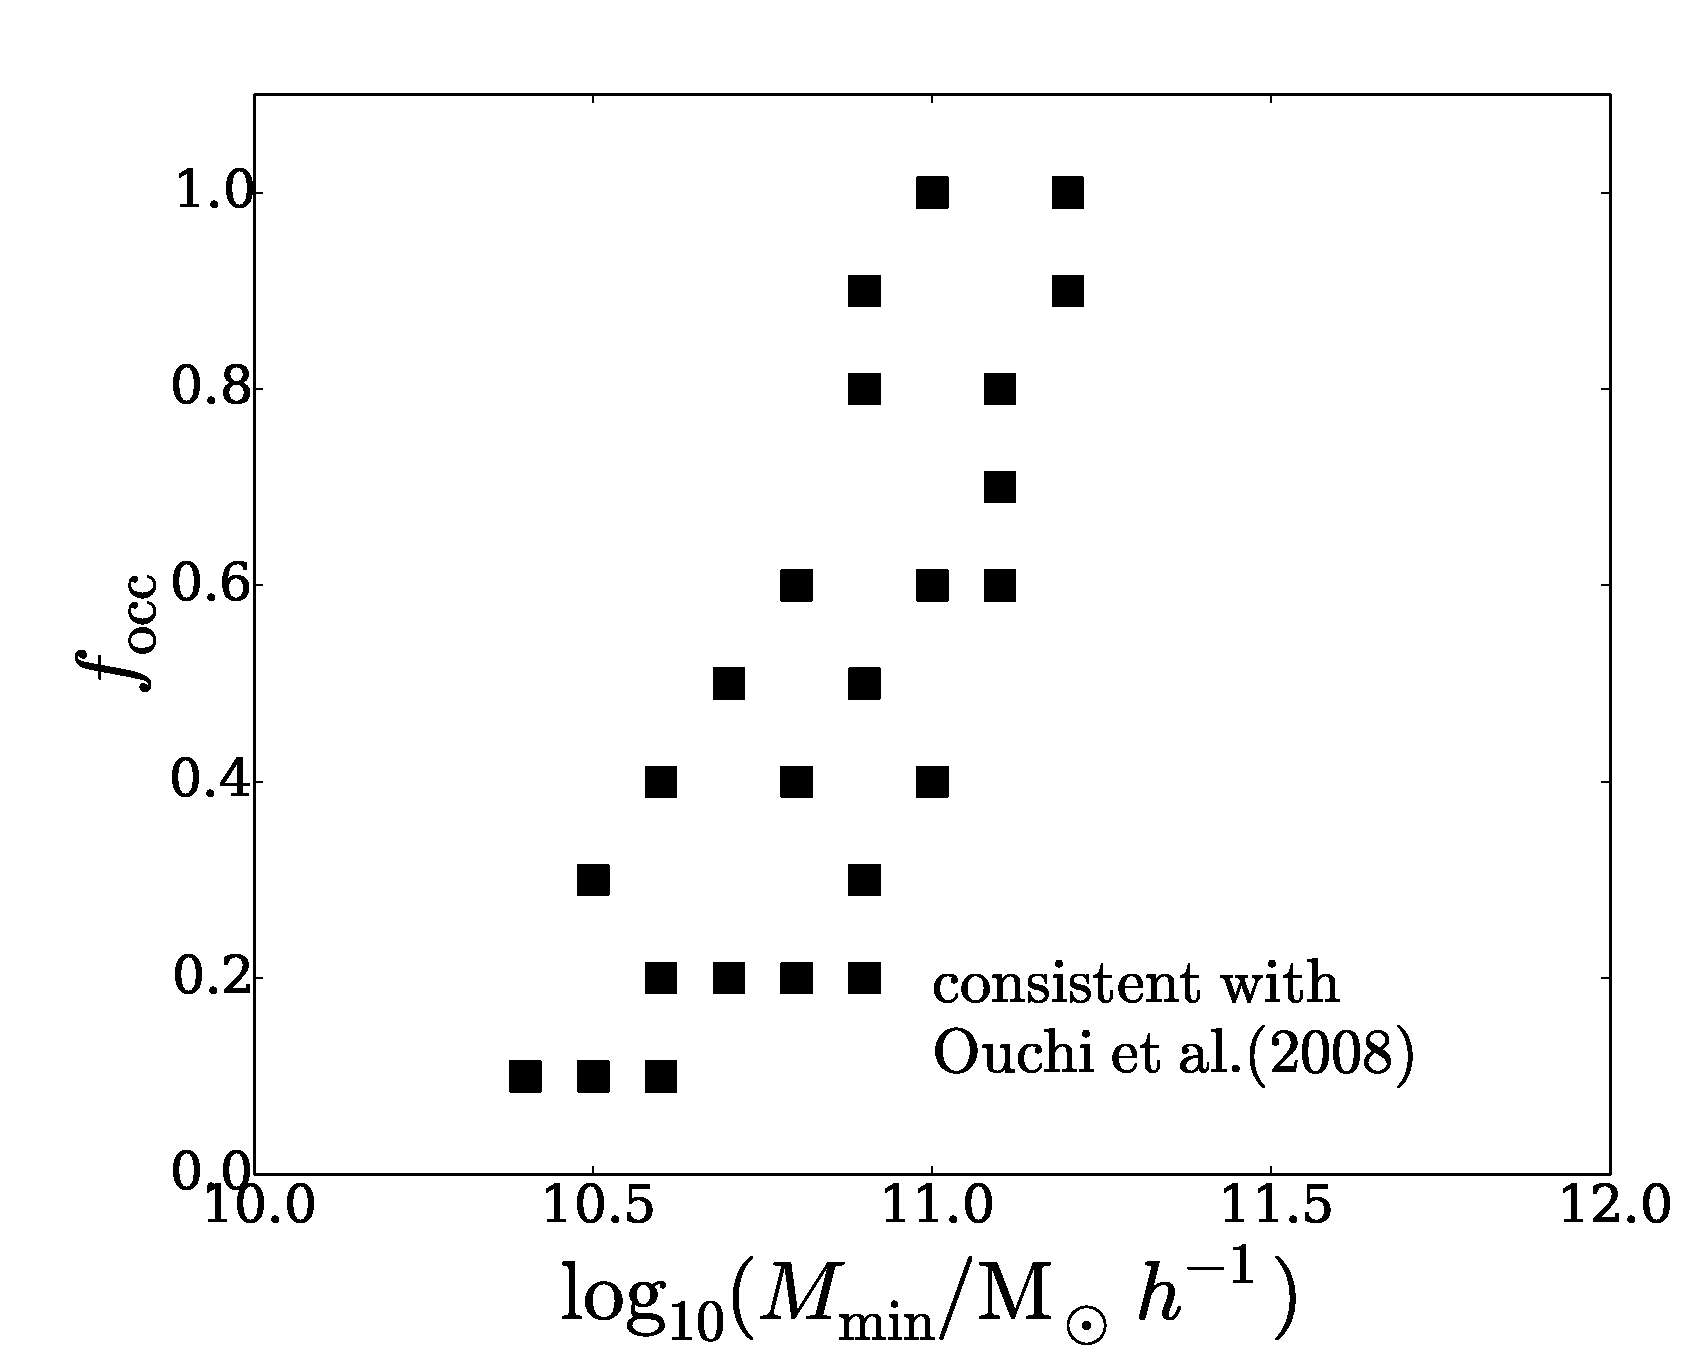
\includegraphics[width=0.46\linewidth,angle=0]{Fig6_f_occ.pdf}
\end{center}
\caption{Planes $M_{\rm min}$-$M_{\rm max}$ (left) and $M_{\rm
    min}$-$f_{\rm occ}$ (right). with the models fulfilling both
   constraints on the maximal number of consistent mocks and the
  angular correlation function. The observational data corresponds to
  \citet{Ouchi2010}.   
  \label{fig:restriction_mock_and_f_occ_corr}} 
\end{figure*} 



Out of the initial set of $9000$ models we end up with $40$ that are
consistent with the observational constraints. To facilitate the
discussion of these models we define a new quantity, the halo mass
range $\Delta M=\log_{10}M_{\rm max} - \log_{10}M_{\rm  min}$, which
together with the occupation fraction, $f_{\rm occ}$, and the minimum
mass $M_{\rm min}$ allows us to classify all the successful models into
three families:     
  

\begin{itemize}
\item[(1)] Low occupation fraction $f_{\rm occ}\leq 0.2$ and narrow
  mass range $\Delta M\leq 1.0$ 
  dex: 16 models. 
\item[(2)] High occupation fraction $f_{\rm occ}> 0.2$ and
  narrow mass range $\Delta M\leq 1.0$: 17 models 
\item[(3)] Low occupation fraction $f_{\rm occ}\leq 0.2$ 
  and wide mass range $\Delta M>1.0$: 7 models
\end{itemize}


A complete parameter list for the three families is presented in Tables
\ref{table:firstfamily}, \ref{table:secondfamily}  and 
\ref{table:thirdfamily}. 

{\bf The models in the third family are barely consistent with the
  constraints from the ACF. They have mean values of $\theta_0$
  outside the observational uncertainties, but have
  are considered as consistent because their large error bars overlap. These
  models they have another particular feature: their minimum mass is
  exactly $M_{\rm min}=10^{10.9}\hMsun$. Because these models are
  are barely compatible with observations and are a minority of the
  consistent models, we exclude them from the rest of the discussion.}


\subsection{Two relevant features}
There are two interesting features in the remaining two first
families. First, the occupation fraction can take any value from $0.1$
to $1.0$. Second, the halos hosting LAEs all have a narrow mass range
$\Delta M\leq 1.0$.  


{\bf The existence of models with high occupation fractions $f_{\rm
    occ}>0.2$ is unexpected from previous clustering analysis that do
  not take  account the effect of cosmic variance in the same way we
  propose in this \documentname. Nevertheless, the mass range
  predicted by our models is consistent with already published
  observational results. This suggests that taking explicitly cosmic
  variance into account hinders the possibility of constraining the
  LAEs occupation fraction.}  

{\bf Concerning the narrow mass range $\Delta M
  <1.0$ the question arises of how can we give a physical
  interpretation for the existence of such  a narrow mass range. We
  can start with a reasonable   assumption. Namely that star formation
  rate increases with halo's  mass.}

Under this assumption the cut at the low mass end, $M_{\rm min}$, can be
interpreted in terms of the minimal star formation rate required to
produce a \ly luminosity above observational detection thresholds.  
A cut at higher halo masses $M_{\rm  max}$ requires a
different justification. There are two complementary physical
scenarios that could provide 

One scenario can be presented in terms of a decreasing escape fraction
of \ly radiation in massive systems. Detailed galaxy formation models
support the idea that massive galaxies with higher metallicities have
larger dust contents and a less concentrated ISM than lower mass
systems. Due to the resonant nature of the \ly line the probability of
absorption  of \ly photons increases in massive systems, producing
high absorption of the \ly line but not of UV continuum or other
non-resonant lines \citep{Laursen2009,ForeroRomero2011}. In a second
scenario larger systems have more extended gaseous envelopes which due
to resonance effects of the \ly line, induces a low surface brightness
and a broader line, making these systems less observable in narrow
band filter surveys \citep{Laursen2009,Zheng2010}.    


\subsection{Comparison to other clustering estimates}

Observational evidence based on the ACF inferred from photometric
measurements in the Extended Chandra Deep Field South has shown that
the median dark matter masses of halos hosting LAEs is
$\log_{10}M_{\rm  med}=10.9^{+0.5}_{-0.9}$\Msun, with a corresponding
occupation fraction of $1-10\%$  \citep{Gawiser07}.  \cite{Ouchi2010}
presents analysis of LAE observations in the redshift interval
$3.1<z<7.0$ and at $z=3.1$ They quote an average mass for the host
dark matter halos of $M_{h}=2.9^{+24.0}_{-2.9}\times 10^{10}$ \hMsun
with a corresponding duty cycle of $0.008\pm 0.03$.  

Our results are in a general good agreement with those estimates for
the host mass. This is not completely unexpected given that we have
also required consistency with ACF measurements. These expectations
are {\bf mostly} matched by the first family of models, also summarized in Table
\ref{table:firstfamily}. These models, which favor only the 
low occupations fractions, are also consistent in that regards with
the observational expectations.

The novelty in our results is that we have a detailed estimate for 
host halo mass range together with the escape fraction. This allows us
to show that the halo mass range can, in some cases, be narrow $\Delta M <
0.3$dex, something that cannot be inferred from ACF analysis alone.
Furthermore, In contrast to \citep{Gawiser07} and \citep{Ouchi2010} we
find that an ACF analysis on a single data-set is not enough to rule
out models with a high occupation fraction $f_{\rm occ}>0.3$, which
represent half of our best models. 



\begin{table}
\begin{center}
\begin{tabular}{cccc}\hline\hline
$\log_{10}M_{\rm min}$ & $\log_{10}M_{\rm max}$ & $f_{\rm occ}$ & $\Delta M$\\\hline
 10.4 &10.7 & 0.1& 0.3 \\
 10.5 &10.9 & 0.1& 0.4 \\
 10.5 &11.0 & 0.1& 0.5 \\
 10.6 &10.8 & 0.2& 0.2 \\
 10.6 &11.2 & 0.1& 0.6 \\
 10.6 &11.3 & 0.1& 0.7 \\
 10.6 &11.4 & 0.1& 0.8 \\
 10.6 &11.5 & 0.1& 0.9 \\
 10.6 &11.6 & 0.1& 1 \\
 10.7 &11.0 & 0.2& 0.3 \\
 10.8 &11.2 & 0.2& 0.4 \\
 10.8 &11.3 & 0.2& 0.5 \\
 10.8 &11.4 & 0.2& 0.6 \\
 10.9 &11.9 & 0.2& 1.0 \\
 10.9 &11.7 & 0.2& 0.8 \\
 10.9 &11.8 & 0.2& 0.9 \\\hline
\end{tabular}
\end{center}
\caption{\label{table:firstfamily}
List of parameters for the first
  family of models. Narrow mass range $\Delta M\leq 1.0$ dex and low
  occupation fraction $f_{\rm occ}\leq 0.3$.} 
\end{table}


\begin{table}
\begin{center}
\begin{tabular}{cccc}\hline\hline
$\log_{10}M_{\rm min}$ & $\log_{10}M_{\rm max}$ & $f_{\rm occ}$ & $\Delta M$\\\hline
 10.5 &10.6 & 0.3 & 0.1 \\
 10.6 &10.7 & 0.4 & 0.1 \\
 10.7 &10.8 & 0.5 & 0.1 \\
 10.8 &10.9 & 0.6 & 0.1 \\
 10.8 &11.0 & 0.4 & 0.2 \\
 10.9 &11.0 & 0.8 & 0.1 \\
 10.9 &11.0 & 0.9 & 0.1 \\
 10.9 &11.1 & 0.5 & 0.2 \\
 10.9 &11.3 & 0.3 & 0.4 \\
 11.0 &11.1 & 1.0 & 0.1 \\
 11.0 &11.2 & 0.6 & 0.2 \\
 11.0 &11.4 & 0.4 & 0.4 \\
 11.1 &11.3 & 0.7 & 0.2 \\
 11.1 &11.3 & 0.8 & 0.2 \\
 11.1 &11.4 & 0.6 & 0.3 \\
 11.2 &11.4 & 0.9 & 0.2 \\
 11.2 &11.4 & 1.0 & 0.2 \\\hline
\end{tabular}
\end{center}
\caption{\label{table:secondfamily}List of parameters for the second
  family of models. Narrow mass range $\Delta M\leq 0.4 $ dex and high occupation fraction $f_{\rm occ}>0.2$.}
\end{table}


\begin{table}
\begin{center}
\begin{tabular}{cccc}\hline\hline
$\log_{10}M_{\rm min}$ & $\log_{10}M_{\rm max}$ & $f_{\rm occ}$ & $\Delta M$\\\hline
 10.6 &11.7 & 0.1& 1.1 \\
 10.9 &12.0 & 0.2& 1.1 \\
 10.9 &12.1 & 0.2& 1.2 \\
 10.9 &12.2 & 0.2& 1.3 \\
 10.9 &12.3 & 0.2& 1.4 \\
 10.9 &12.6 & 0.2& 1.7 \\
 10.9 &12.8 & 0.2& 1.9 \\\hline
\end{tabular}
\end{center}
\caption{\label{table:thirdfamily}List of parameters for the third
  family of models. Wide mass range $\Delta M> 1.0$ dex and low
  occupation fraction $f_{\rm occ}\leq 0.2$. {\bf These models are barely
  consistent with the constraints from the Angular Correlation
  Function and have been excluded from the main discussion.}} 
\end{table}


\subsection{In the context of abundance matching models}

The abundance matching methods are based on observational results for
Lyman Break Galaxies (LBGs) \citep{Behroozi2013a,Behroozi2013b}.  In
the case of \cite{Behroozi2013a} the minimum halo mass considered to
be relevant in their analysis is $10^{11.4}$\hMsun. They report
stellar mass mass around $(1.0\pm0.3)\times 10^{9.0}$ \hMsun, while
their star formation rate is in the range $0.6\pm 0.2$ \Msun yr$^{-1}$,
which nevertheless are close to the lower bound of values inferred for
LAEs at high redshift \citep{Gawiser2007,Nilsson2009,Pentericci2009}. 

In our results, all the preferred models have a halo mass range lower
than the minimum of $M_{\rm min}<10^{11.4}$\hMsun considered in
abundance matching at $z=3$. Our results confirm the expectations
that most of  LAEs are to be found in less massive halos LBG hosts. A
detailed analysis of the spectral and photometric properties of LAEs
coupled to the kind of analysis performed in this paper can be a guide
in the study of the properties of low mass dark matter halos at
$z=3.1$, extending the capabilities of abundance matching methods.

\subsection{Caveats of our method}

There are four caveats for the work presented here that are important
to keep in mind. The first is the  
assumption of a single LAE per dark matter halo. This contradicts the
general expectation of dark matter sub-halos in the simulation to host
satellite galaxies. However, it has been found in analysis based on
the shape of the correlation function \citep{Jose2013b} that satellite
galaxies are not a dominant population, making our initial
approximation a reasonable one. {\bf The lack of close pairs in
  observations is another hint that the observed LAE population matches}
Therefore we conclude that including
the effect of satellite galaxies does not change the main results
reported in this \documentname. 

The second caveat is the precise values for the mass intervals. These
values are quoted from halos defined using a FOF halo
finder. Different halo finders and definitions for the detection
density threshold can yield different masses up to a factor $\sim 2$\citep{More2011}. For 
instance a Friends-of-Friends algorithm with linking length $l=0.20$
times the average inter-particle distance finds halos on average $1.4$
times less massive than halos defined  with an spherical overdensity
algorithm halos \citep{Bolshoi}. Therefore, the mass values for
$M_{\rm min}$ and $M_{\rm max}$ should not be considered exact within
less than $\sim 0.2$ dex.   

{\bf The third caveat is the exact value that was used to turn
  filter values into cosmological volumes. Strictly speaking the
  volume probed is a function of the \ly luminosity. Brighter LAEs
  probe a larger volume than fainter ones \citep{Gronwall07}. A proper
way to account for this effect would require to assign luminosities to
each mock LAE and process them in a similar way as mock
observations. However, we can estimate that under the considerations
presented in \citep{Gronwall07}, one could expect the survey depth to
change at most by a factor of $\sim2$. Considering the dependence
of the number density on halo mass (right panel of Figure 1), such
change in volume could be compensated by different values for the
favored model parameters $M_{\rm  min}$ and $M_{\rm max}$ by about the
same factor of $\sim2$. }

{\bf A fourth caveat is the comparing results for the number density
  statistics and the ACF from surveys with different EW cuts. In this
  sense we highlight againt that the two filters and selection
  criteria used by \citep{Ouchi2008} and \citep{Yamada2012} are only
  slightly different. The median number density in the general fields by
  \citep{Yamada2012} is $0.20$ arcmin$^{-2}$, while in
  \citep{Ouchi2008} is $0.099\pm0.005$ arcmin$^{-2}$. This gives us
  confidence that the two different samples can give a self-consistent picture
  within a factor of $\sim2$ for our studies.}  



\subsection{On the reproducibility of our results}

All the software, raw and processed data to produce the results
and plots in this paper are publicly available in a github
repository \footnote{https://github.com/forero/CosmicVarianceLAES}. Most
of the code to produce the plots can be found as an Ipython notebook
\citep{IPython} in the same repository.



\section{Conclusions}
\label{sec:conclusions}

In this \documentname we look for constraints on the preferred mass
and occupation fraction of dark matter halos hosting Lyman Alpha Emitters at
redshift $z=3.1$ in a $\Lambda$CDM cosmology. We perform this study
paying special attention to the impact of cosmic variance on these
results. To this end we build a large number of mock catalogs matching
observational geometries. The mocks are constructed from a N-body simulation
following a simple recipe to assign a single LAE to each halo. Only
a fraction $f_{\rm occ}$ of halos within a mass range  $M_{\rm
  min}<M_{\rm h}<M_{\rm   max}$ can host a LAE. 

We then proceed with a
thorough exploration of the space of free parameters $M_{\rm min},
M_{\rm max}$ and $f_{\rm occ}$ to find mocks that are consistent with
two observational constraints: the surface number density and the
angular correlation function. Out of the initial $9000$ 
combinations of parameters in the model we find $40$ combination of parameters
consistent with observations.

{\bf We find that the information for the number density constrains
  the minium mass to the range
  $10^{10}\hMsun < M_{\rm min} < 10^{11.5}\hMsun$ while the clustering
  constrains the upper mass $M_{\rm    max} < 10^{12}\hMsun$. However,
  this is insufficient to impose a tight constraint  on the escape
  fraction.} Furthermore, we find that the mass range defined as
$\Delta M=\log_{10}M_{\rm max} - \log_{10}M_{\rm min}$ is always
$\Delta M\leq 1.0$. 

{\bf Our approach has allowed the discovery of possible models that have
been overloooked so far in the literature. A central role in these new
models is played by the wide range of escape fraction values. A wide
range in the escape fraction is unexpected from previous studies that
unanimously favor low values for the occupation
fractions \citep[i.e.][]{Gawiser2007,Ouchi2010}. The larges
innnovation in our analysis is the construction of mock obsevations
that directly explore the impact of cosmic variance, which seems to be
at the root of the large uncertainties in the escape fraction.}

Nevertheless, all the halo mass ranges deduced previous analysis are a
subset of the models we find in this \documentname.  All of our
preferred models support the notion that the most massive halos at
$z=3.1$ do not host detectable LAEs. The existence of a narrow mass
range for halos hosting LAEs, $\Delta  M\leq 1.0$ dex, has two
different explanations at least. The first is having LAEs with a
decreasing \ly escape fraction with increasing mass, the second is
having larger screening effects by neutral Hydrogen around the most
massive systems \citep{Laursen2009,ForeroRomero2011}.    

We also find extreme cases with a very narrow $\Delta M<0.3$, meaning that
there is barely a factor of $\sim 2$ between the minimum and halo
mass. If these models can be confirmed, it would mean a great
challenge for galaxy formation models to explain how is that LAEs can
be hosted in such a narrow range of halo mass.  

In summary, we show that {\bf the currently available spatial
  information of LAEs cannot put a tight constraint on their
  occupation fraction of dark matter halos}. This information can
confidently be used to establish that these galaxies are hosted in low
mass halos with masses within a range spanning less than a factor of
ten. {\bf From the point of view of Dark Energy surveys such as
  HETDEX, the narrow mass range for LAEs can be seen as an advantage,
  due to its simplicity, for their modeling aiming at recovering
  cosmological parameters.} We foresee that the new observations with
new instruments (such as MUSE, Hyper SuprimeCam and HETDEX) covering
larger fields and a wider range of luminosities will be key in reducing cosmic variance and imposing tighter constraints on
the properties of dark matter halos hosting LAEs. At the same time,
additional modeling for \ly radiation transfer is needed to put a
tighter constrain on the \ly escape fraction in high redshift
galaxies, also paying attention to newly framed physical phenomena,
such as the stochasticity \citep{ForeroRomero2013} in the star
formation process, which might play a role in inducing detection
biases in high redshift LAEs. 


\section*{Acknowledgments} 
J.E.F-R thanks the hospitality of Changbom Park and the Korea
Institute for Advanced Study where the first full draft of this paper
was completed. The authors also thank Peter Laursen, Paulina Lira, 
Alvaro Orsi and Mark Dijkstra for helpful comments on the physical
interpretation and presentation of our results. We would
also like to thank the referee for their helpful comments.

J.E.F-R was
supported by the FAPA grant by Vicerrector\'ia de Investigaciones at
Universidad de los Andes. The MultiDark Database used in this paper and the web application providing online access to it were constructed as part of the
activities of the German Astrophysical Virtual Observatory as result
of a collaboration between the Leibniz-Institute for Astrophysics
Potsdam (AIP) and the Spanish MultiDark Consolider Project
CSD2009-00064. The Bolshoi and MultiDark simulations were run on the
NASA's Pleiades supercomputer at the NASA Ames Research Center.



\bibliographystyle{mn2e}
\bibliography{references} 

\end{document}
